\documentclass[12pt]{article}
%\usepackage{paper} %if the document does not compile properly for you on the initial build, uncomment \usepackage{paper} and build again. This should force MikTeX to install package "paper"
\usepackage[margin=1in]{geometry}
\usepackage{float}
\usepackage{natbib}
\bibliographystyle{apsr}
\usepackage{graphicx}
\graphicspath{ {../fig/} }
\usepackage{setspace}
\setstretch{2}
\usepackage[super]{nth}
\usepackage{booktabs}
\usepackage{makecell}
\usepackage{amsmath}
%\usepackage{authblk}
\usepackage{hyperref}
%\usepackage{etoolbox}
%\AtBeginEnvironment{quote}{\singlespacing\small}

\begin{document}

\title{First Year Paper:\\ \large{\citet{iyengar2012affect}}}
\author{Robert Lytle}
\date{\today}
\maketitle
\thispagestyle{empty}
\clearpage
\section{Introduction}
The question ``Has the mass public polarized alongside elites?" has been the subject of an enormous amount of scholarly debate. This debate has been held largely in terms of ideology, with scholars leveraging competing evidence showing \citep{abramowitz2010disappearing} or not showing \citep{fiorina2012disconnect} mass-level polarization. \cite{iyengar2012affect} argue that affect (one's emotional valence towards a stimulus) rather than ideology should be used to evaluate levels of mass polarization. 

While The authors leverage a variety of publicly available observational datasets (further discussed in the body of this work) to demonstrate that Democrats and Republicans exhibit increasing animosity towards out-partisans. In this paper, I replicate the findings of \cite{iyengar2012affect} as they relate to the effect (or lack thereof) of policy preferences on affective polarization, and extend the original work by including both respondents' status as primary voters and their trust in democracy as interaction terms in the model. With primary vote status, I expect to find that policy preferences have a greater effect on out-party affect among primary voters than their non-voting co-partisans. Further, I expect to find similar levels of out-party animus between those who are dissatisfied with democracy and those who are not, but lower levels of warmth toward the in-party on the part of dissatisfied partisans.


\section{Summary of \cite{iyengar2012affect}}
\textit{Affect, Not Ideology} is an ambitious work; seeking to describe the historical trends of affective polarization and to establish a causal chain between hostile media, party-ID, and mass-level affective polarization. This analysis is done in service of the authors' central argument: that Americanist scholars of polarization should study the attitudes of voters towards members of the out-party, not just the ideological differences between opposing parties.

The vast majority of scholars have evaluated polarization in terms of divergent policy preferences between parties and their supporters and have produced contradictory results. While virtually all agree that \textit{elites} have become more polarized, some argue this elite polarization is in response to an increasingly polarized \textit{public} \citep{abramowitz2010disappearing} and some argue against the notion of mass polarization altogether \citep{fiorina2012disconnect, fiorina2005culture}. Still other scholars have argued that observed polarization is not the result of increasingly extreme policy positions on the part of Democrats and Republicans, but the result of previously ideologically heterodox partisans sorting themselves into more appropriate parties \citep{levendusky2009partisan}.

Each of the works discussed in the previous paragraph share a common focus on partisans' \textit{ideology}. Iyengar, Sood, and Lelkes identify this commonality and argue that, since most people have a limited conception of their own ideology \citep{converse1964nature}, and tend to have conflicting \citep{mcclosky1984american} and ideologically incoherent views \citep[p. 76--96]{zaller1992nature}, ideological differences are not a suitable metric by which to gauge mass polarization. In the view of the authors, partisans' affect towards their opponents is a more consistent and substantively meaningful diagnostic of the degree of mass polarization.

To demonstrate this, the authors leverage several existing survey datasets and an advertising dataset\footnote{\textit{ANES Cumulative Study, YouGov/Polimetrix 2008 Election Study}, a \textit{YouGov 2011 multi-national study, Almond \& Verba (1960), Blair Center Election Study}, an \textit{AP Yahoo! News 2008} Election Study and the \textit{Wisconsin Advertising Project}. The implications for validity in using survey data will be discussed in greater detail in section 3.}. The survey data are used first to describe the degree of affective polarization, and are then used in conjunction with the advertisement data to establish a causal link between exposure to hostile political media and affective polarization. Survey data from the United Kingdom is included in the descriptive portion of the research, intended by the authors to serve as a pseudo-control for country-level effects \citep[p. 407]{iyengar2012affect}, comparing a country with parties whose ideology is more salient (the U.K.) to the U.S.

The authors find evidence supporting their claim that the U.S. has undergone a large increase in affective polarization, while the U.K. has polarized ``only modestly" (p. 417) since the 1960s. Further, they find little evidence to suggest the animosity in the U.S. is driven by ideological differences between partisans, contending instead that the ``mere act of identifying with a political party is sufficient to trigger negative evaluations of the opposition" \citep[p. 407]{iyengar2012affect}. Replicating this finding and extending it through a subgroup analysis of party factions and the addition of more recent data will be the principal focus of my paper.

Finally, the authors find support for their claim that exposure to hostile media campaigns strengthens individuals' partisan convictions \citep[p. 407]{iyengar2012affect}, though problems with their finding will be discussed in Section 3.3 of this paper. They close the paper by reiterating their call for a broader investigation of affect by scholars.

In short: \citeauthor{iyengar2012affect} identify a shortcoming in the ongoing debate over the existence of mass-level polarization---that scholars have focused exclusively on partisans' ideology. Instead, they argue that analyses of ideology are insufficient means by which to evaluate mass polarization. The authors argue for a new conception of division: partisans' affect towards their opponents. Iyengar et al. show that partisans are becoming increasingly divided from (and hostile towards) one another and posit that this division is the result of increasingly hostile media, rather than ideological differences between partisans. Therefore, ideological homogeneity between Democrats and Republicans is not sufficient evidence of a broader lack of polarization. I replicate the findings as they relate to the role of ideology in affective polarization, and extend the model to distinguish between groups of primary (non)voters and those who feel dissatisfied with democracy.

\subsubsection{Authors' Model of Affective Polarization}
The core hypothesis (\textit{\textbf{H1}}) of Iyengar et al. is that the U.S. is subject to increasing levels of affective polarization. This polarization, by definition, is dependent \textit{exclusively} on individual level animus towards out-partisans. Working backwards up the causal chain, animus towards the outparty is caused by salient partisan identity (\textit{\textbf{H2}}). The salience of party ID is then increased by politically charged media (\textit{\textbf{H3}}). This chain is represented in \textit{Figure \ref{fig:dag}'s} Directed Acyclic Graph (DAG) by the nodes ``Party ID" and ``Individual-level Out-party Animus" each of which can be both an outcome or exposure variable, depending on the hypothesis in question.

While the descriptive claim \textbf{\textit{H1}} is articulated clearly in the text, the presentation of the causal claims is more muddled; this becomes a problem when attempting to draw causal inferences from the data. These issues result from an imprecise translation of the theoretical data-generating process to statistical causal inference, and are discussed further in Section 3.3.6.

\begin{figure}[h!]
\center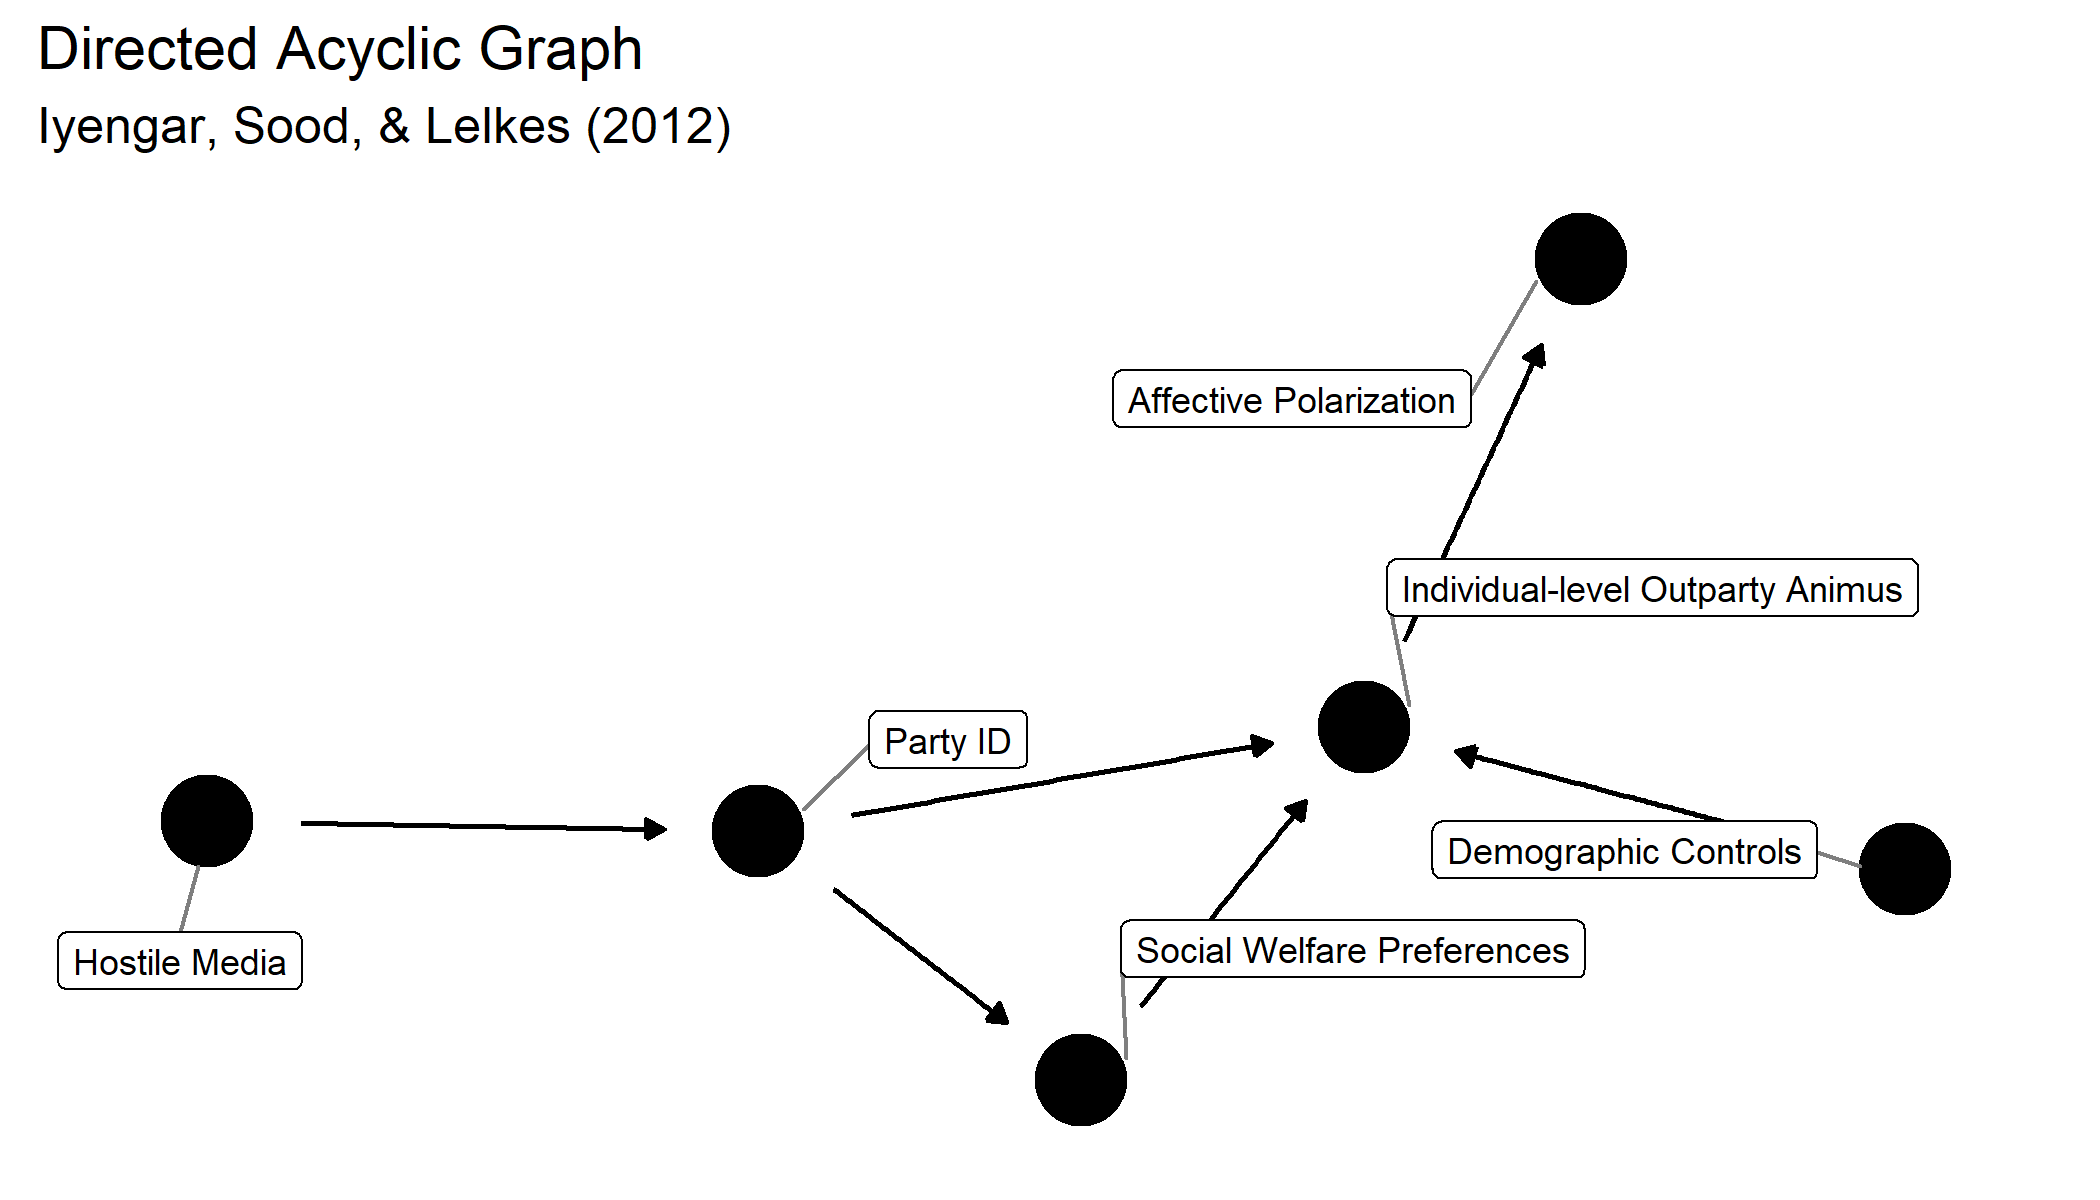
\includegraphics[width=6in]{ext-dag.png}
\caption{\label{fig:dag}\textit{A Directed Acyclic Graph of the causal processes described by \citeauthor{iyengar2012affect}.}}
\end{figure}

Fortunately, the core descriptive claim is both sound and a valuable contribution to the polarization literature. Iyengar et al. show unambiguous and increasingly wide attitudinal cleavages between supporters of the major parties, using a previously under-explored set of measures. While the authors' causal model is flawed, they succeed in showing the existence of a phenomenon which \textit{can} be modeled.

Still, there is more work to be done even on the descriptive front. This study does not address sub-partisan units of political identity, such as self identification as a member of a specific caucus or faction (e.g. progressive, tea-party, alt-right) within the broader party and the implications these identities may have for animus directed at an outgroup. A subgroup analysis along these lines is proposed in section four.

\subsection{Role of Ideology in Affective Polarization}

Ideology, the authors contend, plays a minimal role in driving out-party animus. This conclusion is reached through the application of a Two-Factor Structural Equation Model in which both respondents' cultural positions (gay rights, women's place, and abortion) and their economic positions (social security, healthcare, jobs, essential services) are allowed to affect one of three dependent feeling thermometer variables: in-party, out-party, and the difference of the two. Also included in the regression model are several covariates indicating political interest, whether a respondent is a strong partisan, gender, region (whether a respondent is a southerner), and education. The form of the regression equation is:

\begin{equation}
\begin{split}
\hat{Y} = \alpha + \hat{\beta}_1{\mathit{Culture}} + \hat{\beta}_2\mathit{Econ} + \hat{\gamma}_3\mathit{Strong Partisan} +  \hat{\beta}_4\mathit{Interest} +  \gamma_5\mathit{Female} + \\ \hat{\gamma}_6\mathit{South} + \hat{\gamma}_7\mathit{High School} + \hat{\gamma}_8\mathit{Some College} + \hat{\gamma}_9\mathit{Advanced} + \hat{\gamma}\mathit{interest}*\mathit{internet}
\end{split}
\end{equation}

\noindent where dummy variables are indicated by a gamma coefficient. All variables are rescaled so that the minimum value of each is 0, and the maximum is 1. Missing data are imputed using the 
\texttt{Amelia} and \texttt{mitools} packages in the \texttt{RStudio} software suite. A total of five datasets are generated, containing estimates of missing observations. The OLS model is applied to each dataset, and the estimate of each coefficient is then averaged across the five datasets and reported.

\subsubsection{Levels of Measurement}

Several Independent variables are (arguably) in violation of the assumption of a quantitative or dichotomous independent variable. With the exception of $\mathit{South}$ each IV is constructed from one (or multiple survey questions). $\mathit{Culture}$ and $\mathit{Econ}$ are comprised of questions which ask respondents to rank their degree of support or agreement  for a political or cultural statement. For example: respondents are asked if federal spending on social securit should be increased, kept the same, decreased, or cut entirely. These choices; which are coded as 0, .25, .75, and 1 respectively (most liberal to most conservative); are clearly not quantitative---the size of the interval between each choice is mathematically meaningless---but are nonetheless treated treated as such in the regression model. 

Other variables ask respondents to mark their preferred position on a policy scale, as is \texttt{womensrights} (a component of the culture factor) in which a respondent places themselves somewhere between 1-"women and men should have equal roles" and 7-"a woman's place is in the home". The use of these Likert type items in regression analysis in social science is fairly common and less troubling than variables which consist of a number of discrete choices which are assumed to be a continuous scale in the statistical analysis, but should be treated with caution all the same. It may be wise to adopt a new coding procedure, or to re-specify the ordinal variables as dummies.


\subsubsection{Survey Validity Issues}
\citeauthor{iyengar2012affect} Operationalize inter-partisan affect using two principal measures. The first, ``net partisan affect" (NPA), is the difference between partisans' rating of their in-party and out-party on a feeling thermometer (p. 411). This measure is supplemented with respondents' answer to the question: 
\begin{quote}
``How would you feel if you had a son or daughter who married a Republican/Democrat (Conservative/Labor) supporter? Not at all upset, somewhat upset, very upset?" (p.411)
\end{quote}
Both of these measures are high in content validity, but should still be treated with some caution, dependent as they are on self-assessed survey data. First, it is not clear the degree to which the authors' measures of mass polarization are actually picking up antipathy towards party supporters or party \textit{elites}. The marriage question above clearly asks about ``supporter(s)", but the ANES feeling thermometers are more ambiguous, asking respondents to describe ``people who are Republicans or Democrats" \citep[p. 412]{iyengar2012affect}. In this second example, the elite status of the fictional Republican or Democrat is not specified, and it may not be clear to the respondent (or researcher) what sort of Republican or Democrat the respondent described.

Second, surveys are notoriously vulnerable to issues of framing, priming, and response instability \citep[p. 53--75]{zaller1992nature}, which at best introduce noise in the data and at worst (or at the most interesting, depending on one's perspective) are illustrative of a broader problem with the measurement of public opinion---that many people are simply ``Making it up as [they] go along", to borrow a phrase from Zaller. While these problems are not addressed by \citeauthor{iyengar2012affect} \textit{post facto}; surveys (including the ANES, from which much of these data are drawn) take steps to ameliorate some of the threat from other forms of response bias, often randomizing the order in which questions are asked so as to avoid priming respondents. Still, the larger problem of instability is a more fundamental problem, and one that is not addressed in the text.

A third validity concern of these data is the possibility that respondents have under reported their attachment to their party. As people generally express a preference for bipartisanship \citep{harbridge2014public}, there is logical reason to believe respondents' desire to appear less partisan could lead to Hawthorne effects or social-desirability bias, posing a potential threat to the construct validity of the findings \citep[p. 73, Table 3.1 Item 8]{shadish2002experimental}. Fortunately, if the results are the product of social desirability bias they should \textit{underestimate} the degree of affective polarization. Thus the possibility of unaccounted for social desirability bias does not pose a major threat to the core findings of the paper.


\subsection{Replication}

Below, I present the results of the replication of \citeauthor{iyengar2012affect}. Please note that these tables are placeholders; the final version of this paper will have much more attractive (and readable) figures.
\begin{table}[H]
\begin{table}[H]
\centering
\begin{tabular}{lrrrrl}
\toprule
X1 & results & se & (lower & upper) & missInfo\\
\midrule
(Intercept) & 0.27 & 0.04 & 0.18 & 0.36 & 15 \%\\
CU01r & 0.00 & 0.04 & -0.07 & 0.08 & 12 \%\\
SW01r & 0.02 & 0.05 & -0.06 & 0.11 & 17 \%\\
interest & 0.03 & 0.02 & -0.01 & 0.07 & 6 \%\\
demrep == 1TRUE & 0.06 & 0.02 & 0.03 & 0.09 & 6 \%\\
\addlinespace
genderFEMALE & 0.00 & 0.02 & -0.03 & 0.03 & 3 \%\\
raceWhite & -0.03 & 0.02 & -0.06 & 0.01 & 3 \%\\
south & -0.03 & 0.02 & -0.06 & 0.00 & 8 \%\\
educationCollege or Higher & 0.03 & 0.03 & -0.04 & 0.09 & 2 \%\\
educationHigh school & -0.03 & 0.02 & -0.07 & 0.00 & 5 \%\\
\addlinespace
educationSome college & 0.01 & 0.03 & -0.04 & 0.06 & 3 \%\\
\bottomrule
\end{tabular}
\end{table}
\caption{\label{table} \textit{\textbf{Effect of Cultural (CU01r) and Social Welfare (SW01r) positions on affective polarization for Democrats in 1988}.}}
\end{table}

\begin{table}[H]
\begin{table}[H]
\centering
\begin{tabular}{lrrrrl}
\toprule
X1 & results & se & (lower & upper) & missInfo\\
\midrule
(Intercept) & 0.24 & 0.05 & 0.14 & 0.33 & 11 \%\\
CU01 & -0.03 & 0.04 & -0.10 & 0.04 & 5 \%\\
SW01 & 0.06 & 0.05 & -0.03 & 0.15 & 8 \%\\
demrep == 7TRUE & 0.10 & 0.02 & 0.06 & 0.13 & 7 \%\\
interest & 0.03 & 0.02 & -0.02 & 0.08 & 4 \%\\
\addlinespace
genderFEMALE & -0.03 & 0.02 & -0.06 & 0.00 & 4 \%\\
raceWhite & 0.02 & 0.03 & -0.05 & 0.08 & 4 \%\\
south & 0.02 & 0.02 & -0.01 & 0.06 & 5 \%\\
educationCollege or Higher & -0.04 & 0.04 & -0.11 & 0.04 & 3 \%\\
educationHigh school & 0.01 & 0.02 & -0.04 & 0.05 & 4 \%\\
\addlinespace
educationSome college & 0.01 & 0.03 & -0.04 & 0.06 & 3 \%\\
\bottomrule
\end{tabular}
\end{table}
\caption{\label{table} \textit{\textbf{Effect of Cultural (CU01r) and Social Welfare (SW01r) positions on affective polarization for Republicans in 1988}.}}
\end{table}

\begin{table}[H]
\begin{table}[H]
\centering
\begin{tabular}{lrrrrl}
\toprule
X1 & results & se & (lower & upper) & missInfo\\
\midrule
(Intercept) & 0.13 & 0.08 & -0.02 & 0.29 & 3 \%\\
CU01r & 0.15 & 0.08 & 0.00 & 0.30 & 14 \%\\
SW01r & 0.03 & 0.07 & -0.11 & 0.17 & 19 \%\\
internetTRUE & -0.07 & 0.04 & -0.16 & 0.01 & 9 \%\\
interest & -0.04 & 0.05 & -0.14 & 0.06 & 11 \%\\
\addlinespace
demrep == 1TRUE & 0.14 & 0.02 & 0.10 & 0.18 & 2 \%\\
gender2. Female & 0.02 & 0.02 & -0.01 & 0.06 & 2 \%\\
race50. White (no mention of other race) & -0.04 & 0.04 & -0.11 & 0.03 & 0 \%\\
race88. Don't know & 0.01 & 0.16 & -0.31 & 0.33 & 1 \%\\
race89. Refused & 0.13 & 0.13 & -0.13 & 0.39 & 0 \%\\
\addlinespace
raceOther & -0.08 & 0.04 & -0.15 & 0.00 & 1 \%\\
south & 0.02 & 0.02 & -0.02 & 0.06 & 2 \%\\
educationCollege or Higher & 0.08 & 0.06 & -0.04 & 0.20 & 3 \%\\
educationHigh school & 0.02 & 0.06 & -0.09 & 0.14 & 1 \%\\
educationSome college & 0.06 & 0.06 & -0.06 & 0.17 & 2 \%\\
\addlinespace
internetTRUE:interest & 0.15 & 0.06 & 0.03 & 0.27 & 13 \%\\
\bottomrule
\end{tabular}
\end{table}
\caption{\label{table} \textit{\textbf{Effect of Cultural (CU01r) and Social Welfare (SW01r) positions on affective polarization for Democrats in 2004}.}}
\end{table}


\begin{table}[H]
\begin{table}[H]
\centering
\begin{tabular}{lrrrrl}
\toprule
X1 & results & se & (lower & upper) & missInfo\\
\midrule
(Intercept) & 0.07 & 0.09 & -0.11 & 0.25 & 1 \%\\
CU01 & 0.10 & 0.07 & -0.03 & 0.23 & 4 \%\\
SW01 & 0.17 & 0.07 & 0.04 & 0.30 & 2 \%\\
demrep == 7TRUE & 0.12 & 0.02 & 0.08 & 0.17 & 0 \%\\
interest & 0.12 & 0.06 & 0.00 & 0.23 & 7 \%\\
\addlinespace
internetTRUE & 0.06 & 0.06 & -0.05 & 0.17 & 16 \%\\
gender2. Female & 0.02 & 0.02 & -0.02 & 0.06 & 1 \%\\
race50. White (no mention of other race) & 0.02 & 0.05 & -0.08 & 0.13 & 0 \%\\
race88. Don't know & 0.22 & 0.24 & -0.24 & 0.69 & 1 \%\\
raceOther & 0.02 & 0.07 & -0.12 & 0.15 & 2 \%\\
\addlinespace
south & 0.04 & 0.02 & -0.01 & 0.08 & 0 \%\\
educationCollege or Higher & -0.05 & 0.08 & -0.20 & 0.11 & 2 \%\\
educationHigh school & -0.08 & 0.08 & -0.23 & 0.07 & 1 \%\\
educationSome college & -0.05 & 0.08 & -0.20 & 0.10 & 2 \%\\
interest:internetTRUE & -0.09 & 0.07 & -0.23 & 0.06 & 9 \%\\
\bottomrule
\end{tabular}
\end{table}
\caption{\label{table} \textit{\textbf{Effect of Cultural (CU01r) and Social Welfare (SW01r) positions on affective polarization for Republicans in 2004}.}}
\end{table}

The coefficients reported here are fairly different from those given in \citet{iyengar2012affect} (presented below). I suspect this may be due to some misunderstanding on my part of the multiple imputation and structural equation methods used to create the datasets on which the OLS regression was performed. I will consult with my advisor, as well as one of the co-authors to diagnose the problem.

\begin{figure}[H]
\center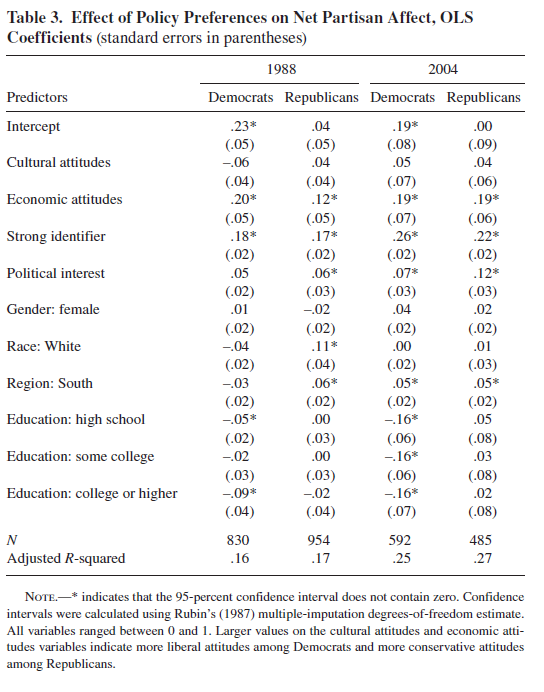
\includegraphics[width=5in]{isl-fig-3.png}
\caption{\label{fig:cdf-avg}\textit{\textbf{The original results from Iyengar, Sood, and Lelkes (2012).} There are inconsistencies between my replication and the original work. It is fairly likely that these are due to the structural equation model and imputation methods employed by the authors.}}
\end{figure}

%\subsection{Research Design Concerns and Limitations}


%\subsubsection{Unit of Analysis}

%\citeauthor{iyengar2012affect} use individual level attitudinal data to make inferences about the state of the broader population. Their primary hypothesis is that the United States exists in an increasingly affective polarized state---a condition which is only possible to achieve through the individual attitudes of many individuals. Referring to the DAG presented in \textit{Figure \ref{fig:dag}}, we see that polarization is wholly dependent on individual out-party animus. In this case it is perfectly legitimate to draw mass level inferences from individual level data.

%\subsubsection{Manipulability \& Randomization}

%Party ID is difficult to manipulate in an observational study. It is conceivable that an experimental design could assign participants a particular party ID in the limited context of that experiment, but given the importance of individuals’ actual party ID there would be reason to doubt the external validity of such a study. 

%Media exposure can be more easily manipulated in an experimental setting, as in \citet{mutz2007effects}, but the external validity of such experiments is questionable, given the differences between media consumption in the laboratory and in more complex information environments. Fortunately, the opportunity to conduct a natural experiment outside of the laboratory environment exists.

%Iyengar et al use residence in a ``battleground state"\footnote{Defined by the authors as ``States with the two parties’ vote difference of less than 5 percent in the 2000 elections...FL, IA, MO, MN, NH, NM, NV, OH, OR, PA, and WI".} as the exposure variable in their regression to capture the effect of hostile media on partisans' affect (p. 424). Greater causal leverage could be gained over the effect of media by instead conducting a natural experiment using a Geographic Regression Discontinuity (GRD) design. Campaign ads are purchased and distributed in ``Designated Market Areas (DMAs)", collections of counties in which a television ad is shown. These DMAs may extend across multiple states \citep{keele2015geographic}. In other words: residents of a non-battleground state $A$ may reside in a DMA which largely services a battleground state $B$. Residents of the DMA in state $A$ will be exposed to the ads targeting state $B$. Residents of state $A$ living outside the DMA will not be exposed to battleground ads.

%In such a GRD design, state $A$ counties in state $B$'s DMA are considered the treatment group, while state $A$ counties \textit{adjacent} to the DMA are considered the control. While individuals likely self-select into states, it is unlikely that residents self-select into particular DMAs \textit{within} those states. Extant scholarship has exploited this as-if random assignment in the study of media and voter turnout \cite{krasno2008televised, huber2007identifying}.





%Designated Media Exposure



%\subsubsection{Implicit Counterfactuals}
%The implicit counterfactual, a condition of weak partisan identity, is not necessarily unrealistic but is \textit{unlikely}. The salience of partisan identity appears to be at a historical high, and the trend does not appear poised to level out any time soon. Still, some researchers have demonstrated experimental interventions which seem to decrease the importance of party ID to participants (Levendusky, Forthcoming). Additionally, both major parties seem to be undergoing a period of increased ideological heterogeneity, with the left and moderate wings of the Democratic party seemingly ascendant and the embrace of Trump by many (but not all) elites in the Republican party. Scholars have argued that internal ideological heterogeneity was a sufficient condition for the (relatively) low salience of party ID through much of the 20th Century \citep{rohde1991parties}; as such, there is reason not to entirely discount the possibility of a return to an era of relatively weak party ID.

%\subsubsection{SUTVA}
%The Stable Unit Treatment Value Assumption (SUTVA) is the assumption that one individual receiving (or not) the treatment condition does not not affect the outcome in other individuals in the study---the effect of $x$ on $i_1$ is the same, regardless of if (or how) individuals $i_2 \ldots i_n$ received the treatment \citep[p. 48]{morgan2015counterfactuals}. 
%SUTVA is violated in this model, with the potential for spillover effects between partisans. While posing problems for causal inference, this SUTVA violation is intrinsic to the study of polarization. Polarization, by definition, implies an in-group and an outgroup; the compositions of which influence the attitudes of the other. 

%The outcome we are interested in is the social distance between individuals $d_n$ and $r_n$ in groups $D$ and $R$. We can expect this effect to vary based on the treatment homogeneity of $D$ and $R$. In other words, the effect produced by one individual’s partisan identity can depend on the identities and the strength of those around her. For a group identity to be salient (and therefore to produce a powerful effect on social distance towards an outgroup) we would expect to find heterogeneity in the outgroup and homogeneity in the ingroup \citep{rohde1991parties}. As noted by the authors of this study (and authors of more recent work) the observed increase in affective polarization has been concomitant with elite-level partisan sorting over the 20th and 21st centuries. 

%\subsubsection{Endogeneity \& Confounders}


%While the \textit{central} hypothesis of this study is largely descriptive, the DAG describing the data-generating process of \citeauthor{iyengar2012affect} is complex---containing several other potential problem areas. The DAG confusion arises because several of the nodes are both exposure and outcome variables. For example, in \textbf{\textit{H2}} party ID is the exposure variable, whereas it is an outcome in \textbf{\textit{H3}}. The authors' theory holds that the media affects affective polarization \textit{only} through its effect on party ID (p. 407), yet the party ID variable is included in the regression equation for media exposure on partisan affect, suggesting possible over control bias.

%There are two possibilities:
%\begin{enumerate}
%\item The theory is correct, and the effect of media has been underestimated due to controlling for a node  in the middle of a causal path \citep{elwert2014endogenous}.
%\item The theory needs to be amended; media effects partisan affect in ways that are not predicated on an increased sense of party ID.
%\end{enumerate}
%In addition to this concern, there is the possibility of over control bias when evaluating the effect of policy preferences on affect, as policy preferences are often endogenous to party ID \citep{druckman2013elite}\footnote{This is also acknowledged in the footnotes on page 422 of \citeauthor{iyengar2012affect}.} This case is not alarming however, as party ID was not included as a variable when regressing affect on policy preferences. While the authors' articulation of their causal claim is problematic, their core descriptive claim (that the United States has increasingly affectively polarized since the mid-\nth{20} century) is unaffected by these problems.

\section{Intra-Party Affect \& Primaries}

In this section, I motivate an extension to \citet{iyengar2012affect}, drawing on partisanship and feeling thermometer data from the ANES-CDF to present time-series trends in Democrats' affect toward their party and the Republican Party. I show, consistent with extant literature, mean out-party feeling thermometers have been decreasing since the late \nth{20} Century. However, the mean feeling thermometers of the parties writ-large do not provide a sufficiently nuanced view of citizens' affect.

\subsection{Internal Division}
Extant scholarship has, in large part, treated the major parties as affectively monolithic; party ID is assumed the least common denominator of political identity. It is also commonly assumed that warmth toward the in-party is (and has been) high across all partisans \citep{iyengar2012affect}. 


 While affective polarization between partisans \textit{is} very high at present, there is also reason to be suspicious of internal divisions \textit{within} each party. \cite{mason2018ideologues} finds that, in addition to partisan identity, citizens hold ideological identities. In other words, individuals see themselves not just as ``Democrats" and ``Republicans", but as ``liberals" and ``conservatives". These  ideological and partisan identities are related to one another, but suggest that political identities which cross cut partisanship are theoretically plausible.

%\begin{figure}[H]
%\center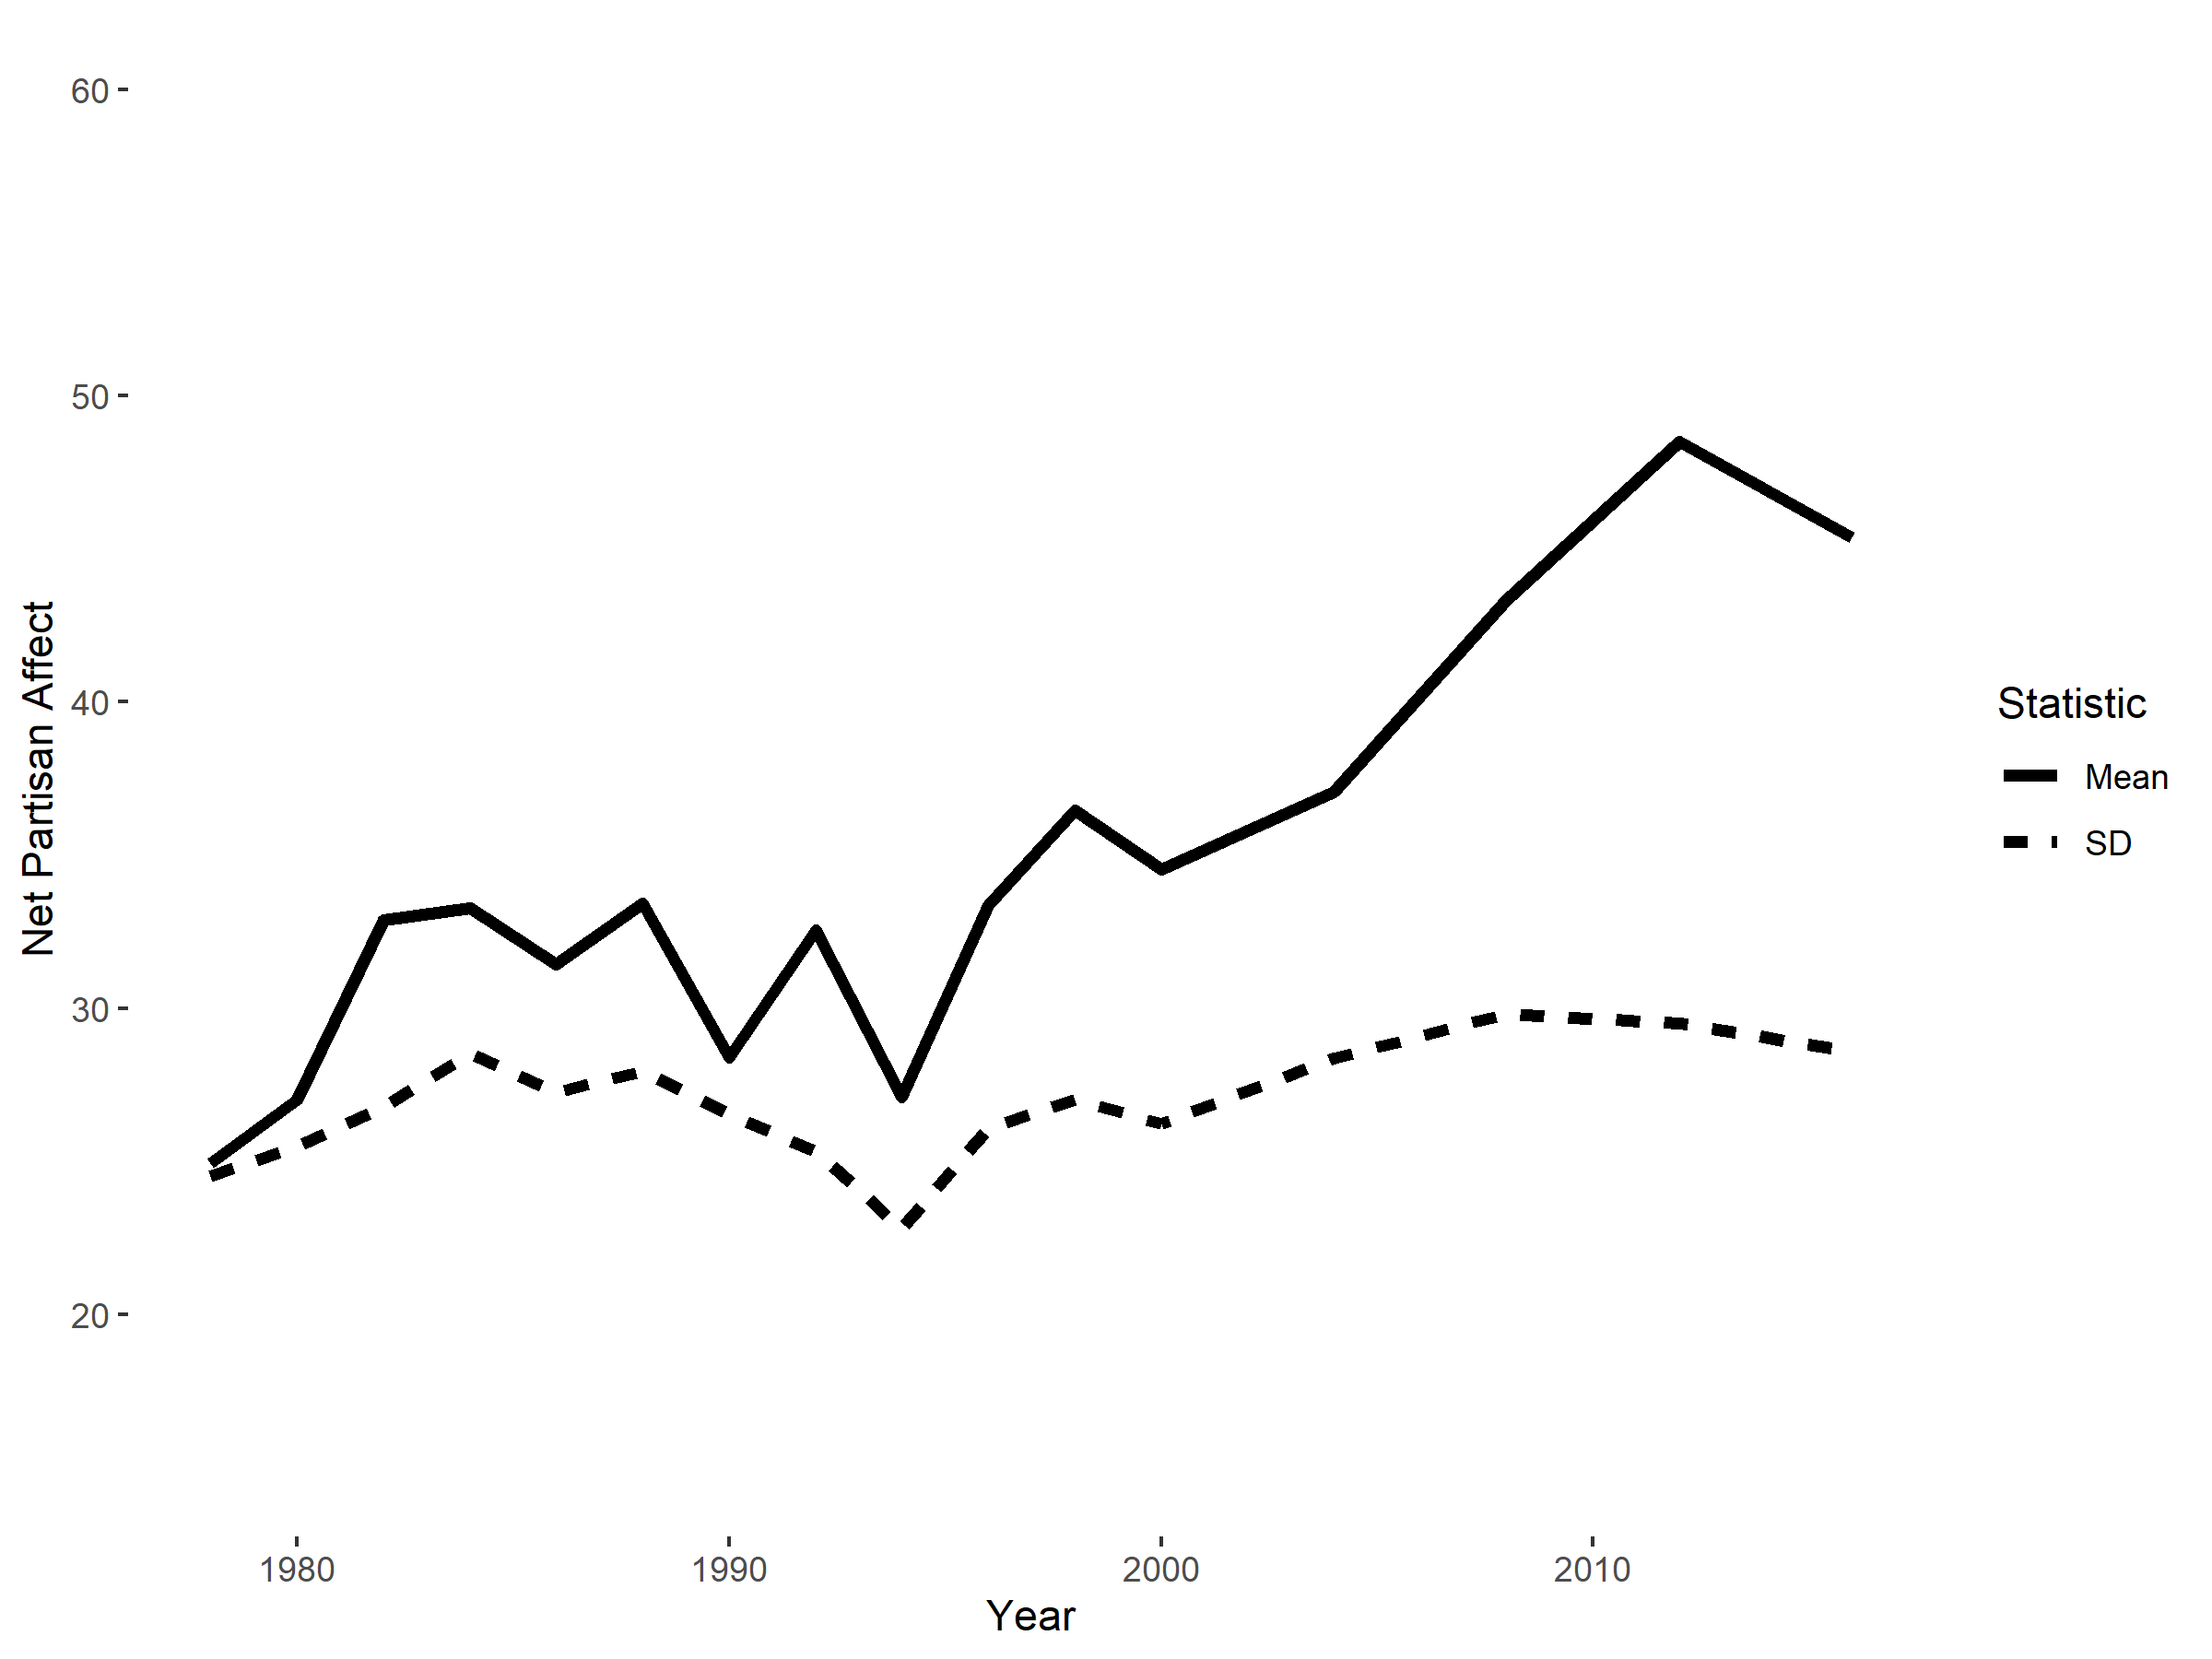
\includegraphics[width=6in]{cdf-npa.png}
%\caption{\label{fig:cdf-npa} \textit{\textbf{Democrats Net Partisan Affect Since 1978.} NPA has increased, but so has the variance. Subtracting in-party FT from out-party FT obscures variation occurring in each measure.}}
%\end{figure}
\begin{figure}[H]
\center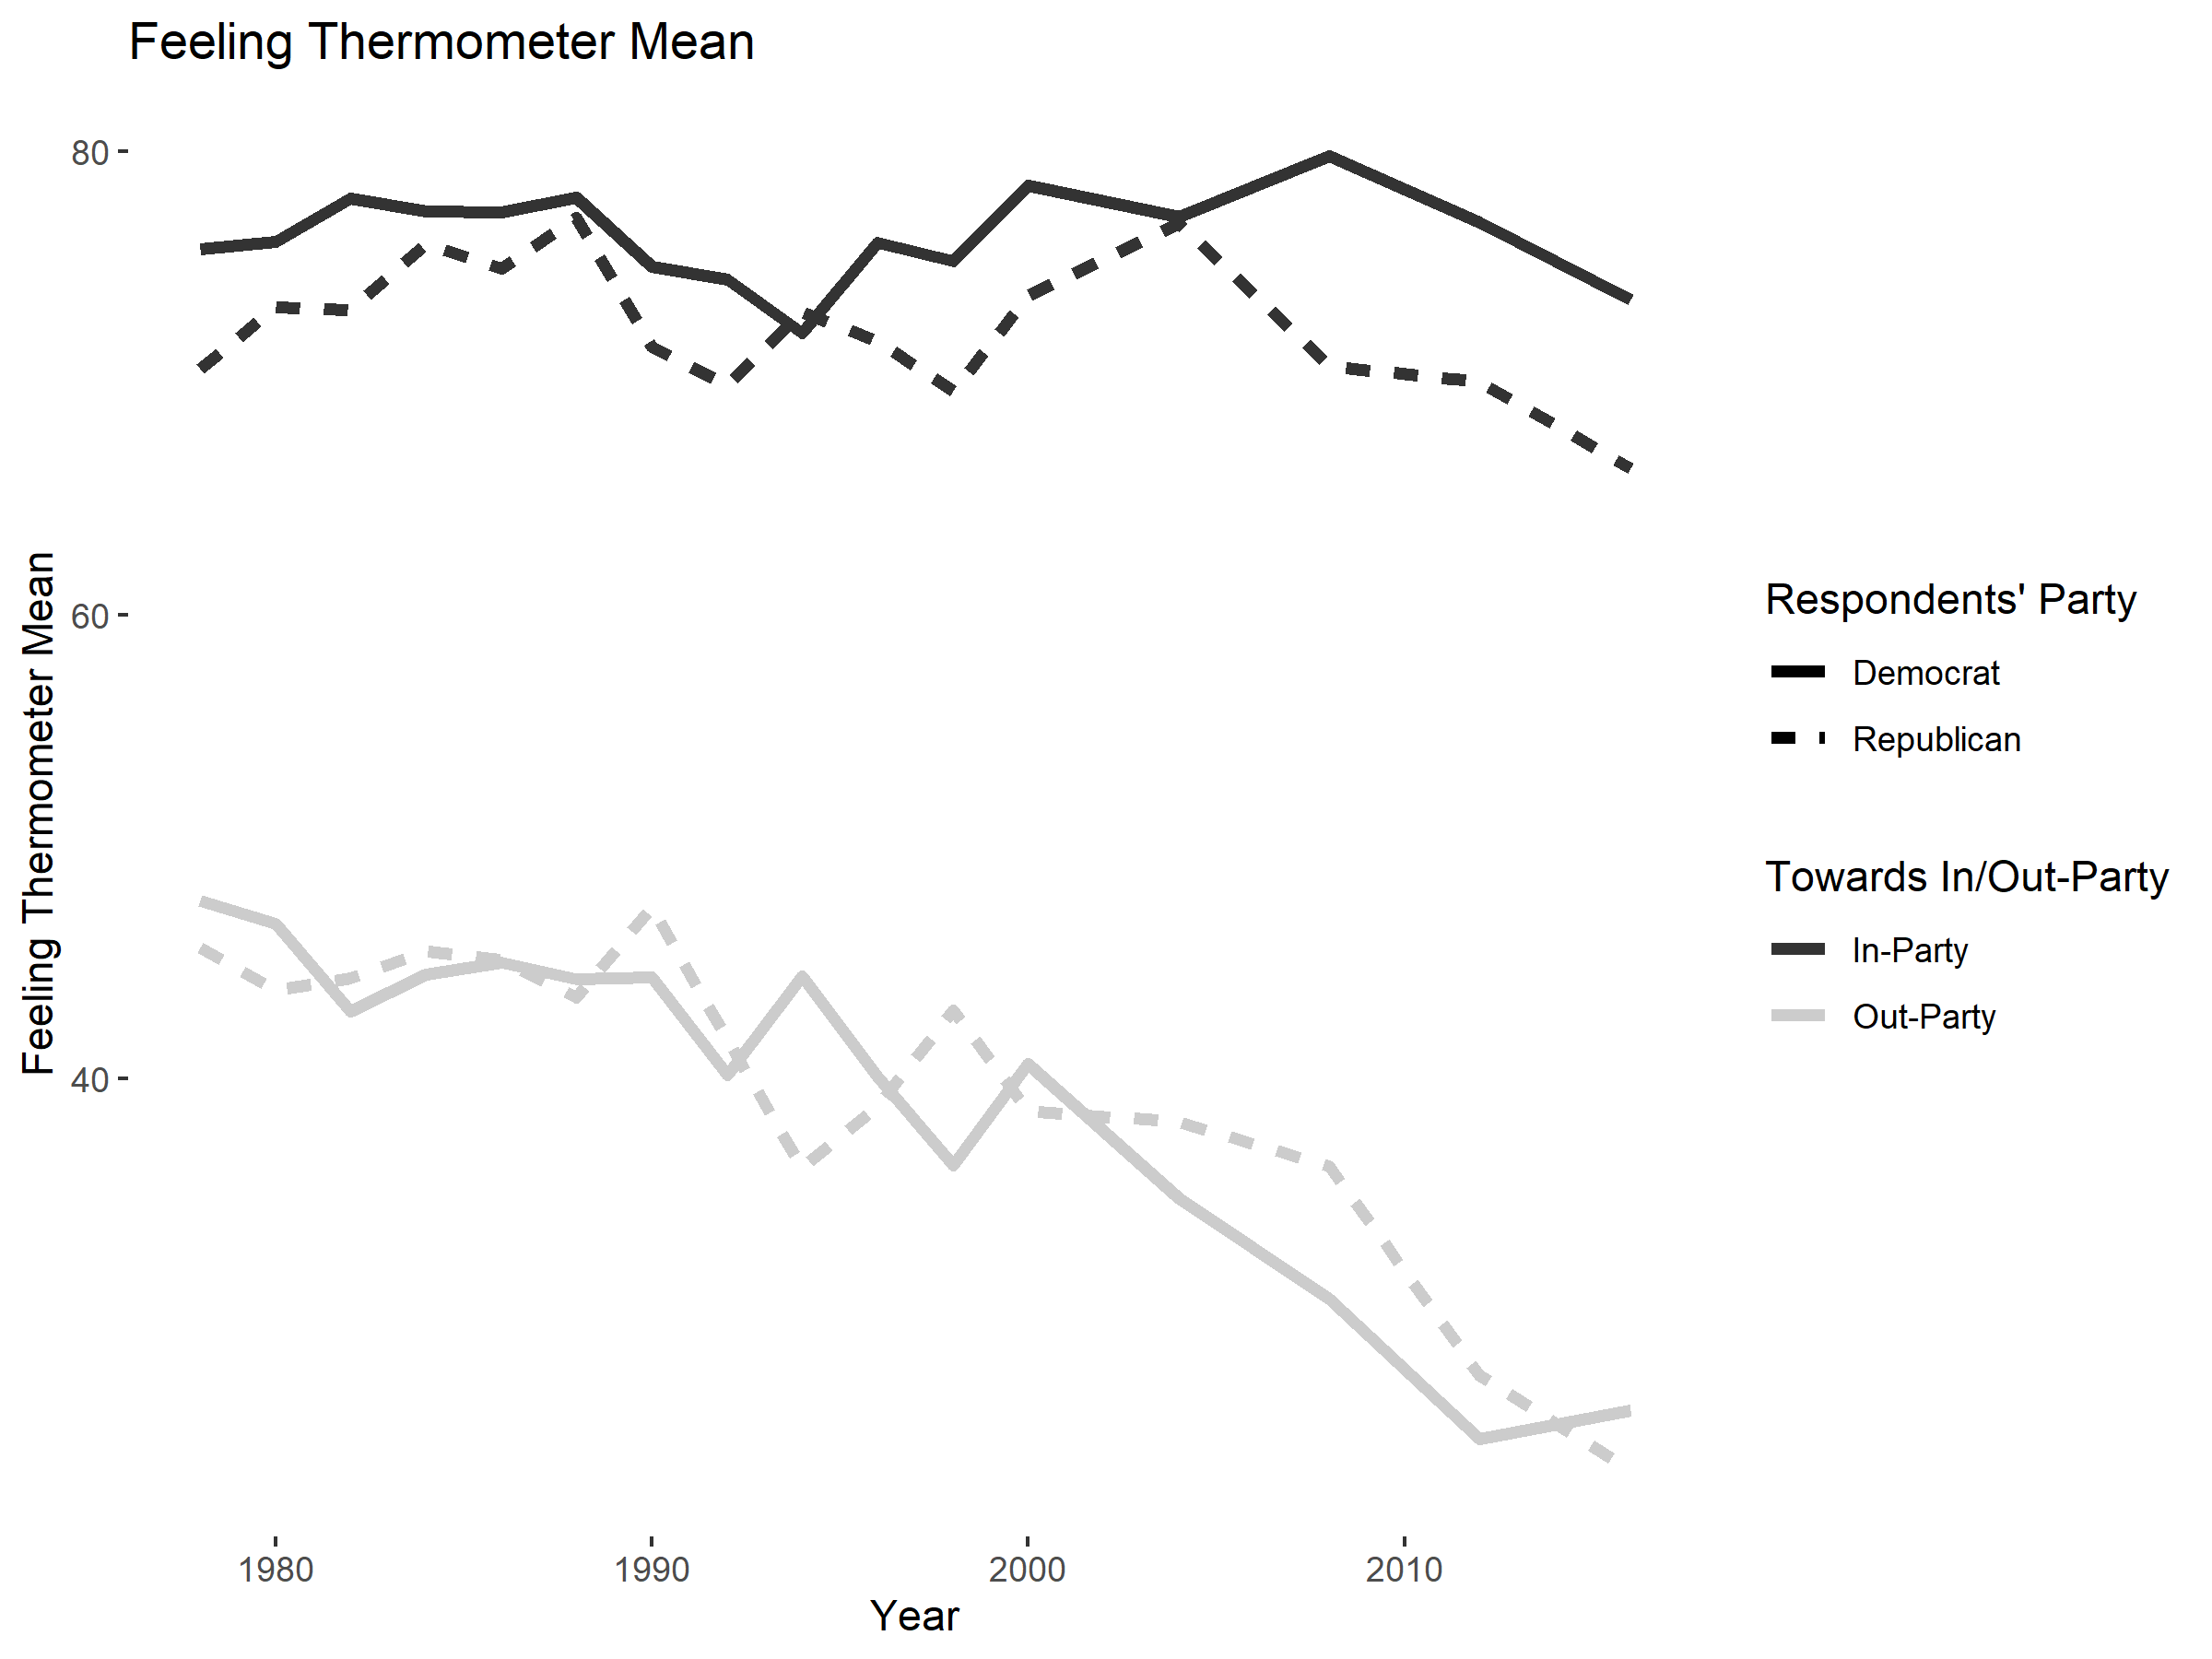
\includegraphics[width=5in]{cdf-avg.png}
\caption{\label{fig:cdf-avg}\textit{\textbf{Yearly mean of partisans' in-party and out-party feeling thermometers, 1978--2016.} Consistent with the extant literature (e.g., \citet{iyengar2012affect}, Democrat and Republican in-party FTs are consistently high (with a slight decrease since the first decade of the 2000s).}}
\end{figure}
\noindent Figure \ref{fig:cdf-avg} shows the average in-party and out-party feeling thermometer for Republicans and Democrats from 1978-2016. We clearly see out-party feeling thermometers scores decline; while the in-party remains relatively constant. This is true of both parties.

Unfortunately reliance on annual means as a description of partisan affect paints too simple a picture. The standard deviation of the feeling thermometers, presented in figure \ref{fig:cdf-sd}, shows that the stability of mean in-party affect observed in Figure \ref{fig:cdf-avg} belies an increase in the variation around that mean. This variation has increased in each iteration of the survey since 2004, both Republicans and Democrats have become less cohesive in their feelings toward their own party than at any other time period for which we have data. It should be noted that, historically, partisans are less cohesive in their feelings towards the out-party, though the variance in intra-party affect now seems to be on par with out-party feelings. %Both figures \ref{fig:cdf-sd} and \ref{fig:cdf-avg}are reproduced in the Appendix using data from Democrat leaning independents, to similar results.

%%%%%%


\begin{figure}[H]
\center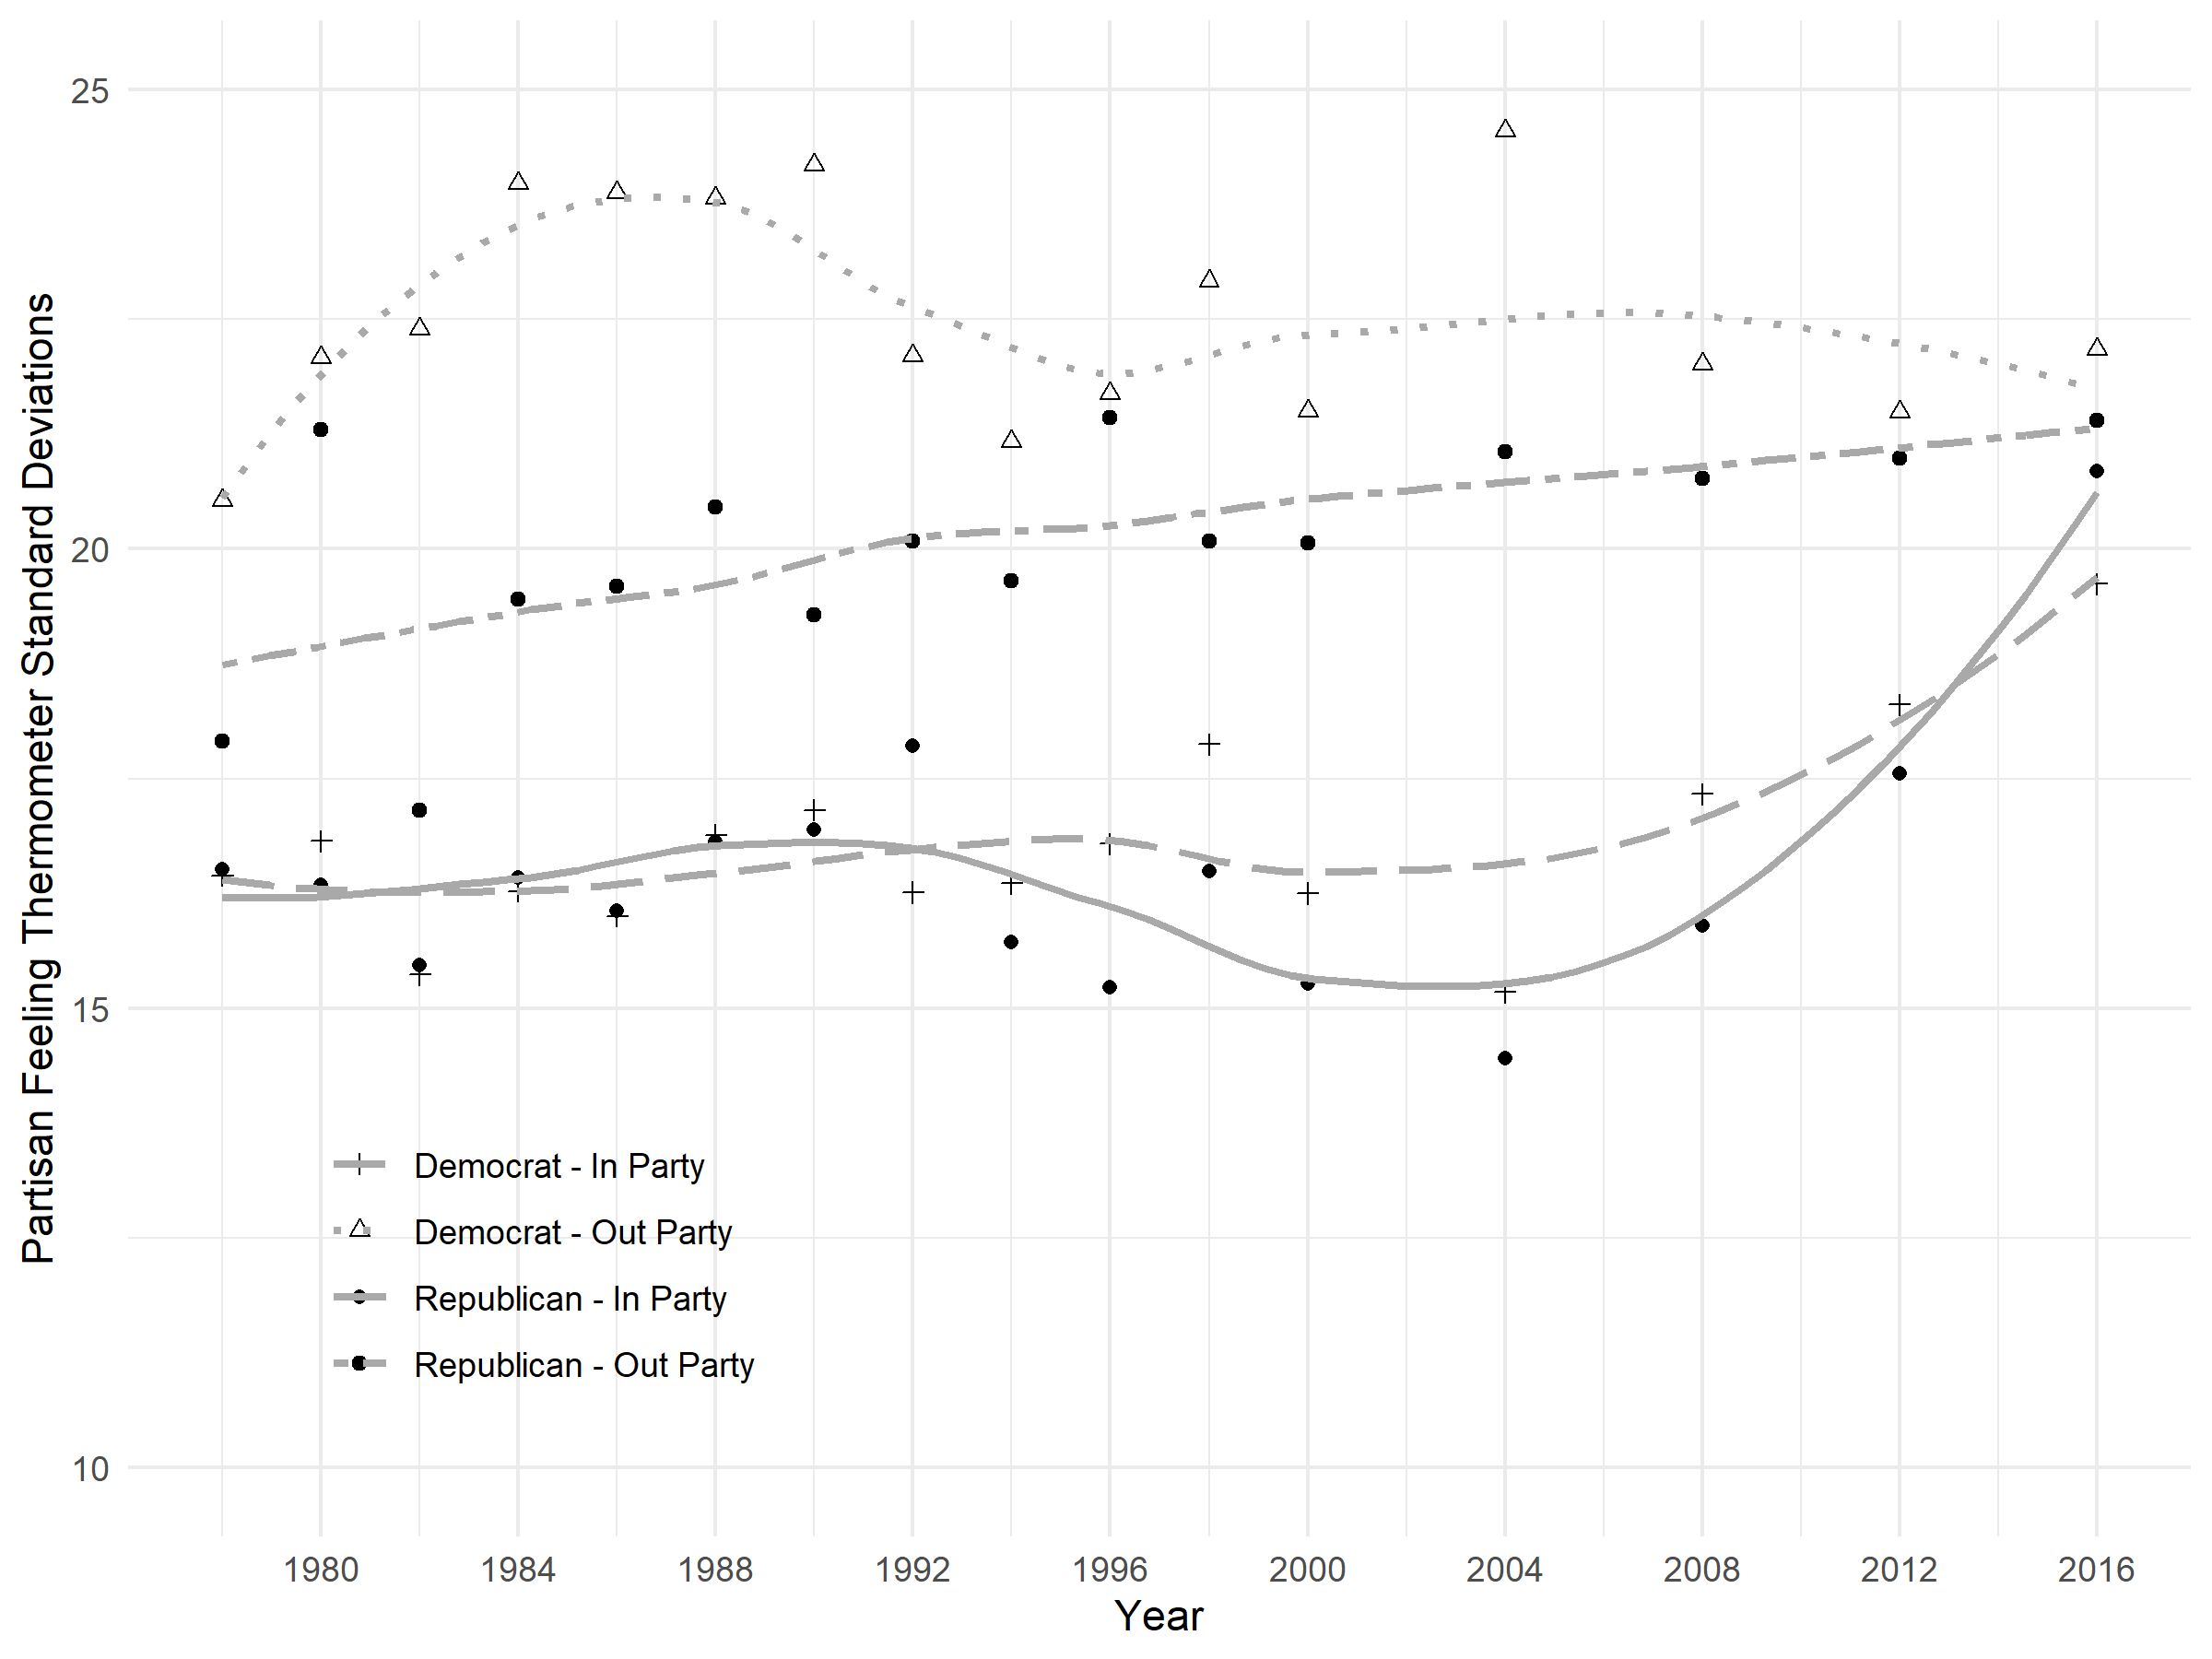
\includegraphics[width=5in]{cdf-sd.png}
\caption{\label{fig:cdf-sd} \textit{\textbf{Standard Deviation of partisans' in party feeling thermometers, 1978--2016.} After several decades of minimal change, the variation in in-party feeling thermometer ratings increased substantially between 2004 and 2016. This change is robust to both the Fligner-Killeen and Levene's tests of homogeneity of variance.}}
\end{figure}
%%%%%



The changes in variance observed above between 2004 and 2016, as well as 1978-2016 are robust to both the Levene's and Fligner-Killeen tests of homogeneity of variances. These tests evaluate the null hypothesis that the variance of a variable between two samples or groups is equal, and are robust to non-normally distributed data. Each tests rejects the null at $p<.05$ (precise p-values to be reported in the appendix).

%\begin{figure}[H]
%\center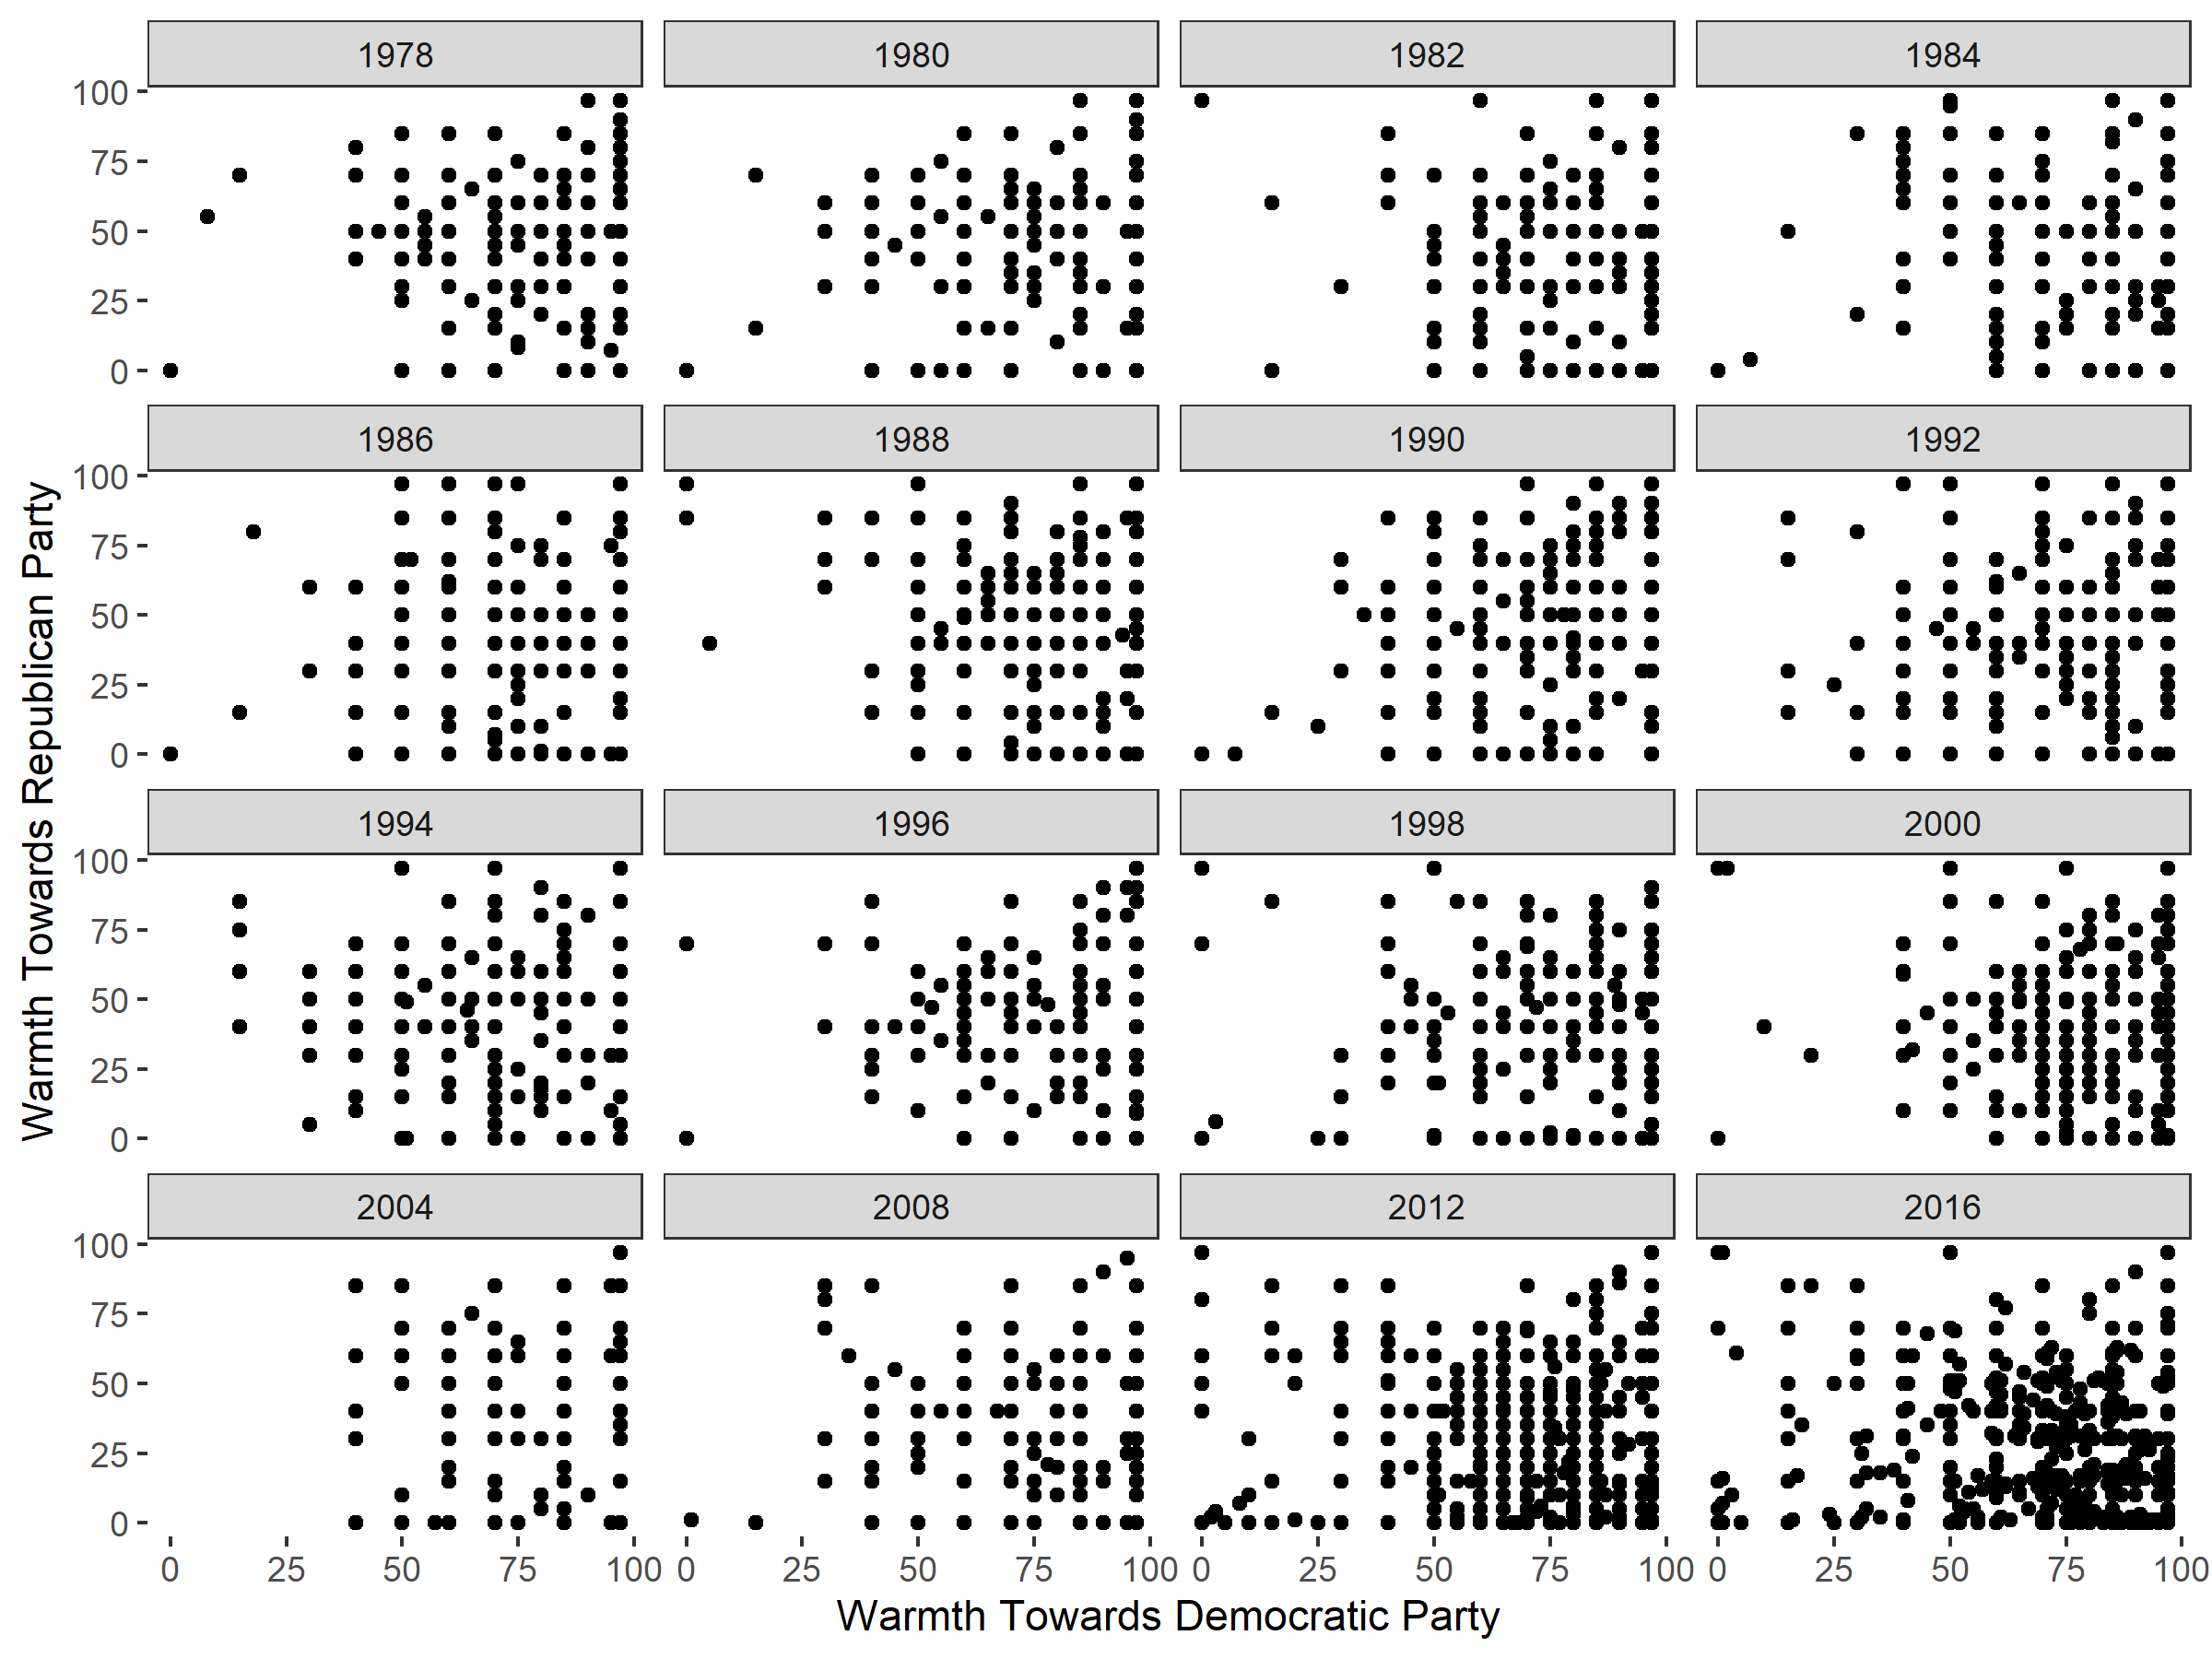
\includegraphics[width=6in]{cdf-scatter-dem.png}
%\caption{\label{fig:cdf-scatter} \textit{\textbf{Scatterplots of Democrats' feeling thermometer scores toward the Democratic and Republican parties from 1978-2016.} Democrats have gotten more cold towards the Republican Party, but an increasing number are also cold towards \textit{both} parties.}}
%\end{figure}

%To visualize the variation described above, I scatterplot Democrats' feeling thermometers towards their in-party and out-party, across all available years. Consistent with the theoretical expectation of \cite{iyengar2012affect}, most respondents have clustered in the bottom right of the plot, indicating warmth towards the Democratic party and coldness towards the Republicans. However, in 2012 and 2016, we also see a striking number of respondents in the bottom left, reporting cold affect towards \textit{both} parties. 

%Using a Levene Test---a statistical procedure which evaluates $H_0: \sigma_1 = \sigma_2$, I show that these data are sufficent to reject the null hypothesis stating that Democrat's in-party and out-party feeling thermometers displayed equal variation in 2004 and 2016. The increase in deviation from 2004, when Democrats were (in recent history) most cohesive, to 2016 at their most dispersed is unlikely to be due to chance. We reject the null hypothesis at $p < .001$, as indicated in the tabe below.

%\begin{table}[H]
%\begin{table}[H]
\centering
\begin{tabular}{>{\raggedright\arraybackslash}p{3cm}>{\raggedleft\arraybackslash}p{3cm}>{\raggedleft\arraybackslash}p{3cm}r}
\toprule
\textbf{ } & \textbf{Df} & \textbf{F value} & \textbf{Pr(>F)}\\
\midrule
group & 1 & 7.423141 & 0.0064838\\
 & 2501 & NA & NA\\
\bottomrule
\end{tabular}
\end{table}
%\caption{\label{table-levene} \textit{\textbf{Results of a Levene Test on the 2004 and 2016 in-party feeling thermometers of Democrats, which indicates meaningful differences in the deviation of the feeling thermometers}}}
%\end{table}
\subsection{A Closer Look At Democrats}

To assess the degree to which systematic differences in affect exist between members of party factions, I present sub-group analyses of primary voters. Primary elections are substantively significant events, allowing partisans a voice in the presentation and direction of their party. In a political environment in which the presidential nominee becomes the de facto leader of the party, the primary process affords non-elite voters a voice in the ideological, political, and stylistic future of the party. The political products offered by primary candidates may reflect (or drive) extant divisions in the party. \cite{wronski2018tale} and \cite{bankert2020authoritarian} find that those scoring highly on measures authoritarian personality traits use their primary vote to ``protect" their party from factions they see as threatening group cohesion. Just as voters do not toss a coin to decide their general election vote, they do not randomly select their choice in the primary; these choices are likely to be meaningful. 

Journalistic accounts of primary elections and their aftermath abound with assertions of internal division and strife within parties after fraught primary election cycles. Democratic primary elections were surprisingly contentious in both 2008 and 2016. In 2008, a particularly brutal primary season spawned the ``Party Unity Means Action" movement (colloquially referred to as the ``Party Unity My Ass" movement) which culminated in an estimated 15-20\% of Clinton supporters voicing their support for John McCain in that year's general election\footnote{\url{https://www.washingtonpost.com/wp-dyn/content/article/2008/06/26/AR2008062604162_pf.html}}.

In 2016 too, primary elections brought to light conflicts between the party's ascendant left-wing and party leadership. These primary divisions seemed to remain salient to engaged voters during the subsequent election for chair of the Democratic National Committee, where Keith Ellison, favored by Sanders supporters lost the race to Obama Secretary of Labor, Tom Perez. Staffers and executives of the 2016 Sanders campaign went on to create groups like \textit{Justice Democrats}, which supports left-leaning candidates in primaries against more centrist Democrats\footnote{Perhaps most notably: \textit{Justice Democrats} supported the campaign of Alexandria Ocasio-Cortez (D-NY), herself a former member of the 2016 Sanders campaign, against former representative Joe Crowley, a high-ranking establishment Democrat.}. 




 

\subsection{Differences in Affect Among Democratic Primary Voters}
I turn now to subgroup analyses of participants and non-participants in the 2008 and 2016 Democratic primaries. I present data from the three largest categories of ANES respondents in each year. In 2008 these were supporters of Barack Obama and Hillary Clinton; in 2016, Hillary Clinton and Bernie Sanders. In each year non-voters made up a majority of respondents.
\begin{table}[H]
\begin{table}[H]
\centering
\begin{tabular}{ll>{\raggedleft\arraybackslash}p{3cm}>{\raggedleft\arraybackslash}p{3cm}>{\raggedleft\arraybackslash}p{3cm}>{}p{3cm}>{}p{3cm}>{}p{3cm}}
\toprule
\textbf{Year} & \textbf{Vote Choice} & \textbf{Net Partisan Affect} & \textbf{Dem Affect} & \textbf{Rep Affect}\\
\midrule
2008 & Didn't Vote & 47.43 & 78.55 & 31.76\\
2008 & Hillary Clinton & 48.37 & 76.51 & 28.14\\
2008 & Barack Obama & 53.63 & 80.40 & 26.77\\
2016 & Didn't Vote & 45.80 & 71.99 & 28.60\\
2016 & Hillary Clinton & 60.19 & 82.62 & 22.48\\
\addlinespace
2016 & Bernie Sanders & 48.34 & 67.70 & 21.45\\
\bottomrule
\end{tabular}
\end{table}
\caption{\label{table} \textit{\textbf{In-party, out-party, and net-affect of supporters of major Democratic primary candidates.} Other candidates have been excluded due to very low sample size. These data are filtered by party-ID; all respondents are Democrats.}}
\end{table}
In 2008 Democrats were largely warm to the party, with averaged feeling thermometers toward their own party in the high 70s or low 80s, in the case of Obama supporters. Clinton voters profess the lowest NPA (identical to that of Bernie voters' in 2016). Consistent with the observed increase in variation, Clinton and Obama voters' net party affects were more similar than those of Clinton and Sanders supporters in 2016.

As expected, affect toward toward republicans dropped across voters and non-voters between 2008 and 2016.  That year, Clinton voters' NPA was substantially higher than that of any other group, and their warmth toward the Democratic party is the highest of all six groups. Bernie voters' net affect is much lower, at about 48. Examining affect toward the Democratic and Republican parties individually, it is clear that Bernie voters' low NPA is the product of coldness towards the Democratic party on the part of Sanders supporters, rather than any particular warmth towards the Republicans. Bernie supporters reported both the lowest in-party thermometer rating (15 points lower than Clinton supporters in 2016) and the lowest out-party score, a point colder towards Republicans than Clinton voters.

\begin{figure}[H]
\center
\includegraphics[width=6in]{primary-scatter.png}
\caption{\label{fig:primary-scatter} \textit{\textbf{Scatterplots of 2008 and 2016 Democratic primary voters Democrat and Republican feeling thermometers.} Mean Democratic feeling thermometer for all groups in each year indicated by vertical line.}}
\end{figure}

When viewing scatterplots of the data presented in table 1, the differences between each group are immediately apparent---particularly in 2016. In 2008, Obama supporters were uniformly warm to the Democratic Party, not a single respondent reported a feeling thermometer below 50. Hillary supporters skewed somewhat colder, but were still generally warm to the Democrats. 

Turning to 2016, Most Hillary supporters were overwhelmingly warm to their party. Bernie voters, on the other hand, are much more ambivalent toward their party. Sanders supporters more closely resemble non-voters from 2016 than any other group in the data. They were less likely than their co-partisans to rate their in-party affect a full 100 and not a single one of those who did rated Republicans above a 25.

Democrats' in-party affect is more heterogenous than has been suggested by existing literature. Variation in Democrats' in-party affect has been increasing since 2004, while mean in-party affect has remained relatively constant, indicating that increasing numbers of Democrats are quite warm to their party, while other groups are lukewarm, or even cold. It is more appropriate to say that Democrats' in-party affect has polarized somewhat, than that to simply claim that it has remained stable.

%
%The data presented above suggest a more complicated picture of Democrats' affect than annual averages would suggest, more suggestive of modest polarization than the stability of opinion insinuated by simple annual averages. It is not that Democrats on the whole feel the same way about the party today as they did in the 1980s, but that some have grown warmer to the party while other have grown colder. In short, Democrats are polarizing---albeit modestly---in their feelings of their own party.


 A potential explanation for these findings is that losing a primary election causes supporters of the losing candidates to dislike the party. Hillary supporters were most cold toward the party in 2008, as were Bernie supporters in 2016. It is also possible that some primary candidates bring new voters into the party, who may not be as friendly towards the organization as existing partisans. This hypothesis seems particularly likely in the case of Sanders in 2016, who did particularly well with those identifying as leaning independents. These hypotheses could be evaluated using panel data to track respondents' changes in partisanship over time.

Finally, the role of ideology in primary vote choice and affect should also be further investigated. While \cite{iyengar2012affect} argue that ideology plays only a minor role in shaping peoples' affective responses, it may be more prevalent among primary voters, who are particularly engaged and attuned to politics \citep{iyengar2012affect}. The affective cleavages between opposing primary voters may be the product of substantive differences on the issues. It is also possible that primary voters chosen candidate functions as an element of their political identity. Possessing a social identity necessitates an in-group and an out-group \citep{brewer2001many}. If a Sanders supporter thinks of their in-group as other Sanders supporters rather than the party writ-large, they may be predisposed to see the party (whose elites overwhelmingly supported Clinton) as a hostile out-group. 

\section{Extension to \citet{iyengar2012affect} }

In order to begin assessing the differences in covariate effects between primary voters I propose an extension to \citet{iyengar2012affect} by way of the addition of two independent variables to their models: a multi-category dummy variable for primary vote choice and two interaction terms. The first interaction term is comprised of a vote for a losing candidate and a dummy variable indicating whether or not a respondent is disatisfied with democracy, the second is cultural preferences interacted with a vote for either candidate---intended to assess whether the cultural concerns of those who vote in a primary are relevant in shaping their partisan affect. Additionally, I would like to extend the analysis to the 2016 iteration of the ANES, in which case the modified functional form of the original model would be as follows:
\begin{equation}
\begin{split}
\hat{Y} = \alpha + \hat{\beta}_1{\mathit{Culture}} + \hat{\beta}_2\mathit{Econ} + \hat{\gamma}_3\mathit{Strong Partisan} +  \hat{\beta}_4\mathit{Interest} +  \hat{\gamma_5}\mathit{Female} + \\ \hat{\gamma}_6\mathit{South} + \hat{\gamma}_7\mathit{High School} + \hat{\gamma}_8\mathit{Some College} + \hat{\gamma}_9\mathit{Advanced} + \hat{\gamma}_{10}\mathit{interest}*\mathit{internet} + \\
\hat{\gamma}_{11}\mathit{Clinton} + \hat{\gamma}_{12}\mathit{Sanders} + \hat{\gamma}_{13}\mathit{Sanders}*\mathit{dissatisfaction} +\hat{\gamma}_{14}\mathit{dissatisfaction} +\\ \hat{\gamma}_{15}\mathit{Culture}(\mathit{Clinton} + \mathit{Sanders})  ,
\end{split}
\end{equation}

\noindent where ``non-voter" is the reference category for primary vote choice. And the dependent variables on which the covariates are regressed are in-party, out-party, and net affect.

 While this specification will not help us to assess the degree to which depressed intra-party affect precedes or is preceded by a primary loss, inclusion of the dissatisfaction interaction term may help to rule out a sore loser effect---it would be difficult to argue that a loss in a primary caused a decrease in in-party FTs if those who voted for the loser and were dissatisfied with democracy showed \textit{greater} warmth to their party. However, I suspect that those who vote for a loser and who are dissatisfied with democracy will exhibit a substantially lower intra-party affect than those who vote for a winning candidate or are satisfied. Additionally, I expect that cultural concerns will increase out-party animosity among primary voters, but have little effect on their in-party feelings.
 
\subsection{Data}

The data necessary to complete this extension are simple to gather, being acquired from the ANES-CDF and the 2016 iteration of the study, which asks respondents for whom they cast a vote in the primary election. As for democratic satisfaction, the ANES asks respondents to rate their satisfaction as "very" or "somewhat" satisfied or dissatisfied with democracy. I will recode those responses who indicate either level of dissatisfaction as a 1.

%\begin{figure}[H]
%\center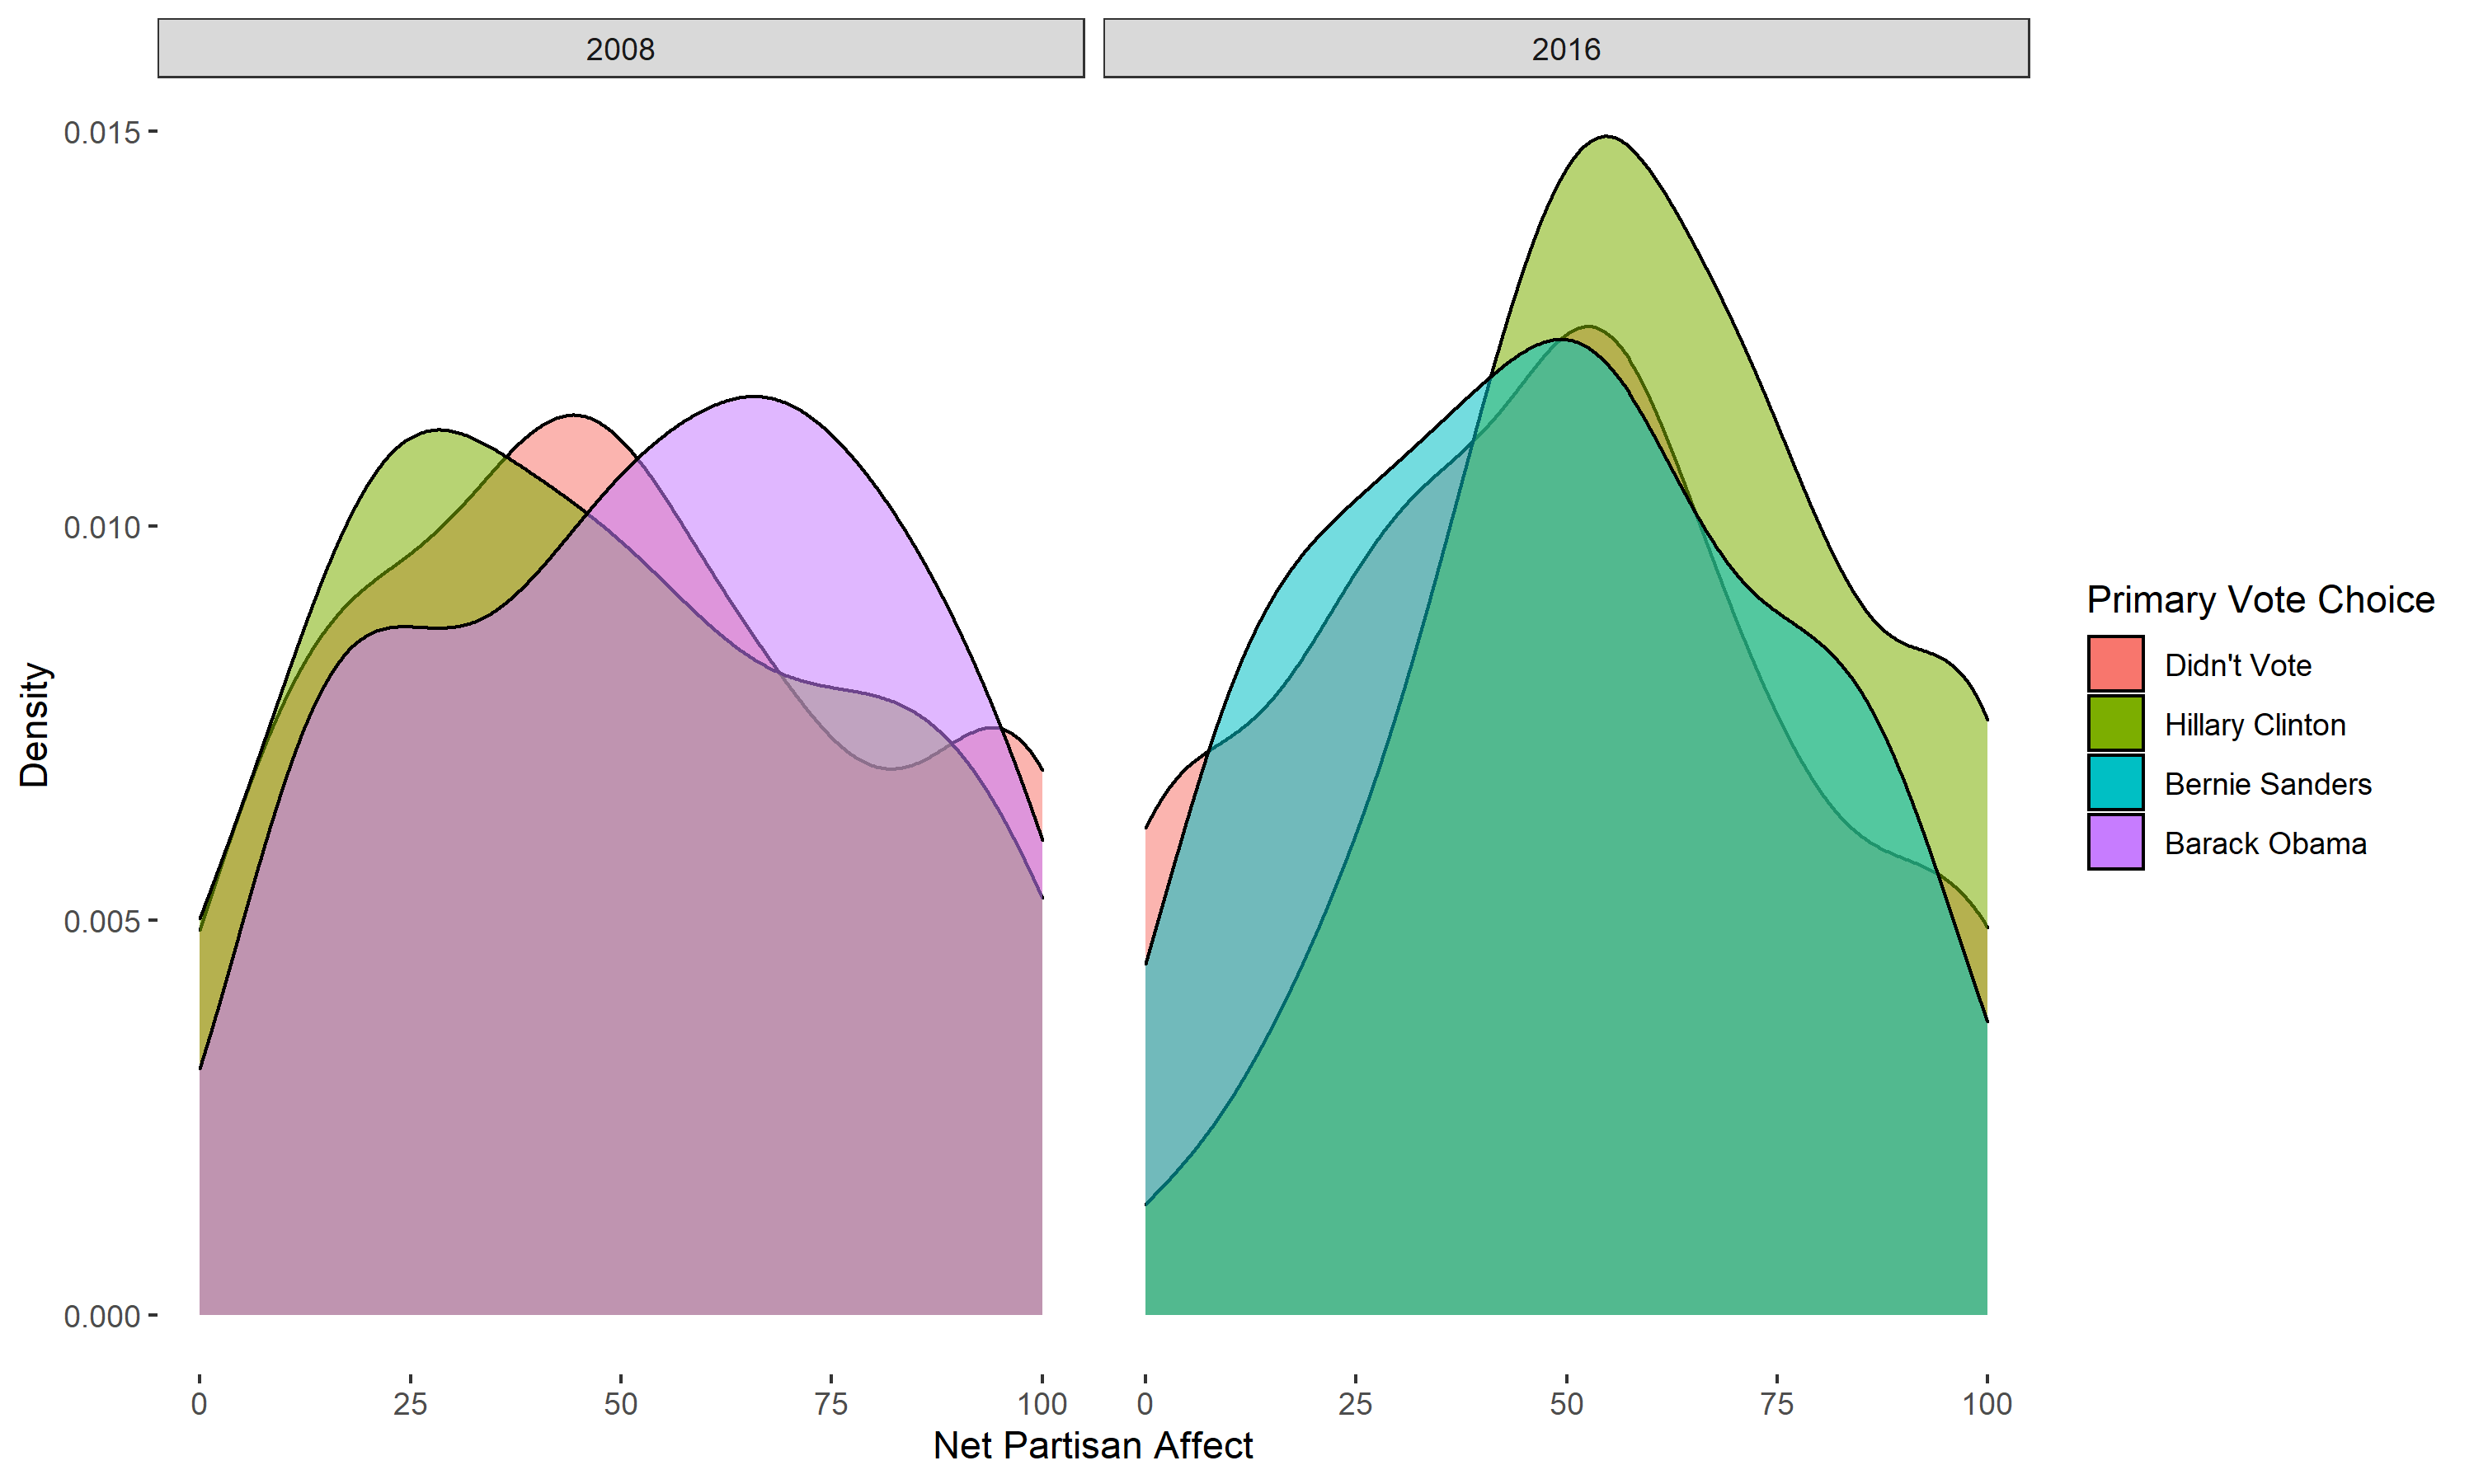
\includegraphics[width=6in]{therm-hist-2016.png}
%\caption{\label{fig:dens}\textit{Density plots of net partisan affect by vote in primary elections}.}
%\end{figure}

%These data are obviously quite limited, looking at members of one party across two years, but they should motivate additional research.


%compare decrease in NPA of losers to average NPA decrease of losers.

%Any observational evaluation of ideological strength is problemmatic because most self-assessments of ideology are typically one-dimensional---asking respondents for their ideological position, but not their \textit{commitment to} that position. Investigating activism may be a useful work-around to this problem. While activists tend to be more extreme than non activists, it would be foolish to believe that \textit{all} activists are more extreme than \textit{all} non-activists. Given these features of ideology, it would be particularly valuable to examine differences in affective polarization between activists and non-activists of similar ideology scores.


\thispagestyle{empty}
\clearpage
\setstretch{1}
\bibliography{references}
\section{Appendix}


\end{document}

%